% Options for packages loaded elsewhere
\PassOptionsToPackage{unicode}{hyperref}
\PassOptionsToPackage{hyphens}{url}
\PassOptionsToPackage{dvipsnames,svgnames,x11names}{xcolor}
%
\documentclass[
  ignorenonframetext,
]{beamer}
\usepackage{pgfpages}
\setbeamertemplate{caption}[numbered]
\setbeamertemplate{caption label separator}{: }
\setbeamercolor{caption name}{fg=normal text.fg}
\beamertemplatenavigationsymbolsempty
% Prevent slide breaks in the middle of a paragraph
\widowpenalties 1 10000
\raggedbottom

\usepackage{amsmath,amssymb}
\usepackage{iftex}
\ifPDFTeX
  \usepackage[T1]{fontenc}
  \usepackage[utf8]{inputenc}
  \usepackage{textcomp} % provide euro and other symbols
\else % if luatex or xetex
  \usepackage{unicode-math}
  \defaultfontfeatures{Scale=MatchLowercase}
  \defaultfontfeatures[\rmfamily]{Ligatures=TeX,Scale=1}
\fi
\usepackage{lmodern}
\usetheme[]{AnnArbor}
\usecolortheme{dolphin}
\usefonttheme{structurebold}
\ifPDFTeX\else  
    % xetex/luatex font selection
\fi
% Use upquote if available, for straight quotes in verbatim environments
\IfFileExists{upquote.sty}{\usepackage{upquote}}{}
\IfFileExists{microtype.sty}{% use microtype if available
  \usepackage[]{microtype}
  \UseMicrotypeSet[protrusion]{basicmath} % disable protrusion for tt fonts
}{}
\makeatletter
\@ifundefined{KOMAClassName}{% if non-KOMA class
  \IfFileExists{parskip.sty}{%
    \usepackage{parskip}
  }{% else
    \setlength{\parindent}{0pt}
    \setlength{\parskip}{6pt plus 2pt minus 1pt}}
}{% if KOMA class
  \KOMAoptions{parskip=half}}
\makeatother
\usepackage{xcolor}
\newif\ifbibliography
\setlength{\emergencystretch}{3em} % prevent overfull lines
\setcounter{secnumdepth}{-\maxdimen} % remove section numbering

\usepackage{color}
\usepackage{fancyvrb}
\newcommand{\VerbBar}{|}
\newcommand{\VERB}{\Verb[commandchars=\\\{\}]}
\DefineVerbatimEnvironment{Highlighting}{Verbatim}{commandchars=\\\{\}}
% Add ',fontsize=\small' for more characters per line
\usepackage{framed}
\definecolor{shadecolor}{RGB}{241,243,245}
\newenvironment{Shaded}{\begin{snugshade}}{\end{snugshade}}
\newcommand{\AlertTok}[1]{\textcolor[rgb]{0.68,0.00,0.00}{#1}}
\newcommand{\AnnotationTok}[1]{\textcolor[rgb]{0.37,0.37,0.37}{#1}}
\newcommand{\AttributeTok}[1]{\textcolor[rgb]{0.40,0.45,0.13}{#1}}
\newcommand{\BaseNTok}[1]{\textcolor[rgb]{0.68,0.00,0.00}{#1}}
\newcommand{\BuiltInTok}[1]{\textcolor[rgb]{0.00,0.23,0.31}{#1}}
\newcommand{\CharTok}[1]{\textcolor[rgb]{0.13,0.47,0.30}{#1}}
\newcommand{\CommentTok}[1]{\textcolor[rgb]{0.37,0.37,0.37}{#1}}
\newcommand{\CommentVarTok}[1]{\textcolor[rgb]{0.37,0.37,0.37}{\textit{#1}}}
\newcommand{\ConstantTok}[1]{\textcolor[rgb]{0.56,0.35,0.01}{#1}}
\newcommand{\ControlFlowTok}[1]{\textcolor[rgb]{0.00,0.23,0.31}{\textbf{#1}}}
\newcommand{\DataTypeTok}[1]{\textcolor[rgb]{0.68,0.00,0.00}{#1}}
\newcommand{\DecValTok}[1]{\textcolor[rgb]{0.68,0.00,0.00}{#1}}
\newcommand{\DocumentationTok}[1]{\textcolor[rgb]{0.37,0.37,0.37}{\textit{#1}}}
\newcommand{\ErrorTok}[1]{\textcolor[rgb]{0.68,0.00,0.00}{#1}}
\newcommand{\ExtensionTok}[1]{\textcolor[rgb]{0.00,0.23,0.31}{#1}}
\newcommand{\FloatTok}[1]{\textcolor[rgb]{0.68,0.00,0.00}{#1}}
\newcommand{\FunctionTok}[1]{\textcolor[rgb]{0.28,0.35,0.67}{#1}}
\newcommand{\ImportTok}[1]{\textcolor[rgb]{0.00,0.46,0.62}{#1}}
\newcommand{\InformationTok}[1]{\textcolor[rgb]{0.37,0.37,0.37}{#1}}
\newcommand{\KeywordTok}[1]{\textcolor[rgb]{0.00,0.23,0.31}{\textbf{#1}}}
\newcommand{\NormalTok}[1]{\textcolor[rgb]{0.00,0.23,0.31}{#1}}
\newcommand{\OperatorTok}[1]{\textcolor[rgb]{0.37,0.37,0.37}{#1}}
\newcommand{\OtherTok}[1]{\textcolor[rgb]{0.00,0.23,0.31}{#1}}
\newcommand{\PreprocessorTok}[1]{\textcolor[rgb]{0.68,0.00,0.00}{#1}}
\newcommand{\RegionMarkerTok}[1]{\textcolor[rgb]{0.00,0.23,0.31}{#1}}
\newcommand{\SpecialCharTok}[1]{\textcolor[rgb]{0.37,0.37,0.37}{#1}}
\newcommand{\SpecialStringTok}[1]{\textcolor[rgb]{0.13,0.47,0.30}{#1}}
\newcommand{\StringTok}[1]{\textcolor[rgb]{0.13,0.47,0.30}{#1}}
\newcommand{\VariableTok}[1]{\textcolor[rgb]{0.07,0.07,0.07}{#1}}
\newcommand{\VerbatimStringTok}[1]{\textcolor[rgb]{0.13,0.47,0.30}{#1}}
\newcommand{\WarningTok}[1]{\textcolor[rgb]{0.37,0.37,0.37}{\textit{#1}}}

\providecommand{\tightlist}{%
  \setlength{\itemsep}{0pt}\setlength{\parskip}{0pt}}\usepackage{longtable,booktabs,array}
\usepackage{calc} % for calculating minipage widths
\usepackage{caption}
% Make caption package work with longtable
\makeatletter
\def\fnum@table{\tablename~\thetable}
\makeatother
\usepackage{graphicx}
\makeatletter
\def\maxwidth{\ifdim\Gin@nat@width>\linewidth\linewidth\else\Gin@nat@width\fi}
\def\maxheight{\ifdim\Gin@nat@height>\textheight\textheight\else\Gin@nat@height\fi}
\makeatother
% Scale images if necessary, so that they will not overflow the page
% margins by default, and it is still possible to overwrite the defaults
% using explicit options in \includegraphics[width, height, ...]{}
\setkeys{Gin}{width=\maxwidth,height=\maxheight,keepaspectratio}
% Set default figure placement to htbp
\makeatletter
\def\fps@figure{htbp}
\makeatother
% definitions for citeproc citations
\NewDocumentCommand\citeproctext{}{}
\NewDocumentCommand\citeproc{mm}{%
  \begingroup\def\citeproctext{#2}\cite{#1}\endgroup}
\makeatletter
 % allow citations to break across lines
 \let\@cite@ofmt\@firstofone
 % avoid brackets around text for \cite:
 \def\@biblabel#1{}
 \def\@cite#1#2{{#1\if@tempswa , #2\fi}}
\makeatother
\newlength{\cslhangindent}
\setlength{\cslhangindent}{1.5em}
\newlength{\csllabelwidth}
\setlength{\csllabelwidth}{3em}
\newenvironment{CSLReferences}[2] % #1 hanging-indent, #2 entry-spacing
 {\begin{list}{}{%
  \setlength{\itemindent}{0pt}
  \setlength{\leftmargin}{0pt}
  \setlength{\parsep}{0pt}
  % turn on hanging indent if param 1 is 1
  \ifodd #1
   \setlength{\leftmargin}{\cslhangindent}
   \setlength{\itemindent}{-1\cslhangindent}
  \fi
  % set entry spacing
  \setlength{\itemsep}{#2\baselineskip}}}
 {\end{list}}
\usepackage{calc}
\newcommand{\CSLBlock}[1]{\hfill\break\parbox[t]{\linewidth}{\strut\ignorespaces#1\strut}}
\newcommand{\CSLLeftMargin}[1]{\parbox[t]{\csllabelwidth}{\strut#1\strut}}
\newcommand{\CSLRightInline}[1]{\parbox[t]{\linewidth - \csllabelwidth}{\strut#1\strut}}
\newcommand{\CSLIndent}[1]{\hspace{\cslhangindent}#1}


% logo
\titlegraphic{
\includegraphics[width=4cm]{../000_logos/logo-blue-vertical}}
\logo{\ifnum\thepage>1
\includegraphics[width=0.5cm]{../000_logos/logo-blue-vertical}\fi}

% UMNG: Manual de image institucional

% Colors

% Umng
\definecolor{yellow}{HTML}{fdc600}
\definecolor{red}{HTML}{ee2a24}

% Estudios a Distancia
\definecolor{blue1}{HTML}{12245b}
\definecolor{blue2}{HTML}{767ca6}
\definecolor{blue3}{HTML}{cad2ec}

% Modify items
\setbeamercolor{palette primary}{bg=blue3}
\setbeamercolor{palette tertiary}{bg=blue1}
\setbeamercolor{frametitle}{bg=yellow}

% Hyperlinks
\hypersetup{
  linkcolor=red,
  citecolor=red
}

\makeatletter
\@ifpackageloaded{caption}{}{\usepackage{caption}}
\AtBeginDocument{%
\ifdefined\contentsname
  \renewcommand*\contentsname{Table of contents}
\else
  \newcommand\contentsname{Table of contents}
\fi
\ifdefined\listfigurename
  \renewcommand*\listfigurename{List of Figures}
\else
  \newcommand\listfigurename{List of Figures}
\fi
\ifdefined\listtablename
  \renewcommand*\listtablename{List of Tables}
\else
  \newcommand\listtablename{List of Tables}
\fi
\ifdefined\figurename
  \renewcommand*\figurename{Figure}
\else
  \newcommand\figurename{Figure}
\fi
\ifdefined\tablename
  \renewcommand*\tablename{Table}
\else
  \newcommand\tablename{Table}
\fi
}
\@ifpackageloaded{float}{}{\usepackage{float}}
\floatstyle{ruled}
\@ifundefined{c@chapter}{\newfloat{codelisting}{h}{lop}}{\newfloat{codelisting}{h}{lop}[chapter]}
\floatname{codelisting}{Listing}
\newcommand*\listoflistings{\listof{codelisting}{List of Listings}}
\makeatother
\makeatletter
\makeatother
\makeatletter
\@ifpackageloaded{caption}{}{\usepackage{caption}}
\@ifpackageloaded{subcaption}{}{\usepackage{subcaption}}
\makeatother

\ifLuaTeX
\usepackage[bidi=basic]{babel}
\else
\usepackage[bidi=default]{babel}
\fi
\babelprovide[main,import]{english}
% get rid of language-specific shorthands (see #6817):
\let\LanguageShortHands\languageshorthands
\def\languageshorthands#1{}
\ifLuaTeX
  \usepackage{selnolig}  % disable illegal ligatures
\fi
\usepackage{bookmark}

\IfFileExists{xurl.sty}{\usepackage{xurl}}{} % add URL line breaks if available
\urlstyle{same} % disable monospaced font for URLs
\hypersetup{
  pdftitle={Describing Data},
  pdfauthor={Luis Francisco Gómez López},
  pdflang={en},
  colorlinks=true,
  linkcolor={Maroon},
  filecolor={Maroon},
  citecolor={Blue},
  urlcolor={Blue},
  pdfcreator={LaTeX via pandoc}}


\title{Describing Data}
\author{Luis Francisco Gómez López}
\date{2024-08-01}
\institute{FAEDIS}

\begin{document}
\frame{\titlepage}

\renewcommand*\contentsname{Table of contents}
\begin{frame}[allowframebreaks]
  \frametitle{Table of contents}
  \tableofcontents[hideallsubsections]
\end{frame}

\section{Please Read Me}\label{please-read-me}

\begin{frame}{}
\phantomsection\label{section}
\begin{itemize}
\tightlist
\item
  This presentation is based on (\citeproc{ref-chapman_r_2019}{Chapman
  and Feit 2019, chap. 3})
\end{itemize}
\end{frame}

\section{Purpose}\label{purpose}

\begin{frame}{}
\phantomsection\label{section-1}
\begin{itemize}
\tightlist
\item
  Utilize descriptive statistics and single variable visualization
  techniques for summarizing and exploring a data set
\end{itemize}
\end{frame}

\section{Weekly store data}\label{weekly-store-data}

\begin{frame}{}
\phantomsection\label{section-2}
\begin{itemize}
\tightlist
\item
  \textbf{storeNum}: store identifier
\item
  \textbf{Year}: year identifier
\item
  \textbf{Week}: week as it would appear in the ISO 8601 system (1-52)
\item
  \textbf{p1sales}: units sold of product 1
\item
  \textbf{p2sales}: units sold of product 2
\item
  \textbf{p1price}: price of product 1
\item
  \textbf{p2price}: price of product 2
\item
  \textbf{p1prom}: whether product 1 was promoted (1) or not (0)
\item
  \textbf{p2prom}: whether product 2 was promoted (1) or not (0)
\item
  \textbf{country}: two-letter country codes defined in ISO 3166-1
\end{itemize}
\end{frame}

\begin{frame}[fragile]{}
\phantomsection\label{section-3}
\begin{itemize}
\tightlist
\item
  \textbf{Import data}
\end{itemize}

\tiny

\begin{Shaded}
\begin{Highlighting}[]
\NormalTok{weekly\_store }\OtherTok{\textless{}{-}} \FunctionTok{read\_csv}\NormalTok{(}\AttributeTok{file =} \StringTok{"http://goo.gl/QPDdMl"}\NormalTok{)}
\NormalTok{weekly\_store }\SpecialCharTok{|\textgreater{}} \FunctionTok{head}\NormalTok{(}\AttributeTok{n=}\DecValTok{5}\NormalTok{)}
\end{Highlighting}
\end{Shaded}

\begin{verbatim}
# A tibble: 5 x 10
  storeNum  Year  Week p1sales p2sales p1price p2price p1prom p2prom country
     <dbl> <dbl> <dbl>   <dbl>   <dbl>   <dbl>   <dbl>  <dbl>  <dbl> <chr>  
1      101     1     1     127     106    2.29    2.29      0      0 US     
2      101     1     2     137     105    2.49    2.49      0      0 US     
3      101     1     3     156      97    2.99    2.99      1      0 US     
4      101     1     4     117     106    2.99    3.19      0      0 US     
5      101     1     5     138     100    2.49    2.59      0      1 US     
\end{verbatim}
\end{frame}

\begin{frame}[fragile]{}
\phantomsection\label{section-4}
\begin{itemize}
\tightlist
\item
  \textbf{Transform data}
\end{itemize}

\tiny

\begin{Shaded}
\begin{Highlighting}[]
\NormalTok{weekly\_store }\OtherTok{\textless{}{-}}\NormalTok{ weekly\_store }\SpecialCharTok{|\textgreater{}}
  \FunctionTok{mutate}\NormalTok{(}\AttributeTok{storeNum =} \FunctionTok{factor}\NormalTok{(storeNum, }\AttributeTok{ordered =} \ConstantTok{FALSE}\NormalTok{),}
         \AttributeTok{Year =} \FunctionTok{factor}\NormalTok{(Year, }\AttributeTok{levels =} \DecValTok{1}\SpecialCharTok{:}\DecValTok{2}\NormalTok{, }\AttributeTok{ordered =} \ConstantTok{TRUE}\NormalTok{),}
         \AttributeTok{Week =} \FunctionTok{factor}\NormalTok{(Week, }\AttributeTok{levels =} \DecValTok{1}\SpecialCharTok{:}\DecValTok{52}\NormalTok{, }\AttributeTok{ordered =} \ConstantTok{TRUE}\NormalTok{),}
         \AttributeTok{p1prom =} \FunctionTok{as.logical}\NormalTok{(p1prom),}
         \AttributeTok{p2prom =} \FunctionTok{as.logical}\NormalTok{(p2prom))}
\NormalTok{weekly\_store }\SpecialCharTok{|\textgreater{}} \FunctionTok{head}\NormalTok{(}\AttributeTok{n=}\DecValTok{5}\NormalTok{)}
\end{Highlighting}
\end{Shaded}

\begin{verbatim}
# A tibble: 5 x 10
  storeNum Year  Week  p1sales p2sales p1price p2price p1prom p2prom country
  <fct>    <ord> <ord>   <dbl>   <dbl>   <dbl>   <dbl> <lgl>  <lgl>  <chr>  
1 101      1     1         127     106    2.29    2.29 FALSE  FALSE  US     
2 101      1     2         137     105    2.49    2.49 FALSE  FALSE  US     
3 101      1     3         156      97    2.99    2.99 TRUE   FALSE  US     
4 101      1     4         117     106    2.99    3.19 FALSE  FALSE  US     
5 101      1     5         138     100    2.49    2.59 FALSE  TRUE   US     
\end{verbatim}
\end{frame}

\begin{frame}[fragile]{}
\phantomsection\label{section-5}
\begin{itemize}
\tightlist
\item
  \textbf{Inspect data: the base R way}
\end{itemize}

\tiny

\begin{Shaded}
\begin{Highlighting}[]
\FunctionTok{as.data.frame}\NormalTok{(weekly\_store) }\SpecialCharTok{|\textgreater{}} \FunctionTok{str}\NormalTok{()}
\end{Highlighting}
\end{Shaded}

\begin{verbatim}
'data.frame':   2080 obs. of  10 variables:
 $ storeNum: Factor w/ 20 levels "101","102","103",..: 1 1 1 1 1 1 1 1 1 1 ...
 $ Year    : Ord.factor w/ 2 levels "1"<"2": 1 1 1 1 1 1 1 1 1 1 ...
 $ Week    : Ord.factor w/ 52 levels "1"<"2"<"3"<"4"<..: 1 2 3 4 5 6 7 8 9 10 ...
 $ p1sales : num  127 137 156 117 138 115 116 106 116 145 ...
 $ p2sales : num  106 105 97 106 100 127 90 126 94 91 ...
 $ p1price : num  2.29 2.49 2.99 2.99 2.49 2.79 2.99 2.99 2.29 2.49 ...
 $ p2price : num  2.29 2.49 2.99 3.19 2.59 2.49 3.19 2.29 2.29 2.99 ...
 $ p1prom  : logi  FALSE FALSE TRUE FALSE FALSE FALSE ...
 $ p2prom  : logi  FALSE FALSE FALSE FALSE TRUE FALSE ...
 $ country : chr  "US" "US" "US" "US" ...
\end{verbatim}
\end{frame}

\begin{frame}[fragile]{}
\phantomsection\label{section-6}
\begin{itemize}
\tightlist
\item
  \textbf{Inspect data: the tidyverse way}
\end{itemize}

\tiny

\begin{Shaded}
\begin{Highlighting}[]
\NormalTok{weekly\_store }\SpecialCharTok{|\textgreater{}} \FunctionTok{glimpse}\NormalTok{()}
\end{Highlighting}
\end{Shaded}

\begin{verbatim}
Rows: 2,080
Columns: 10
$ storeNum <fct> 101, 101, 101, 101, 101, 101, 101, 101, 101, 101, 101, 101, 1~
$ Year     <ord> 1, 1, 1, 1, 1, 1, 1, 1, 1, 1, 1, 1, 1, 1, 1, 1, 1, 1, 1, 1, 1~
$ Week     <ord> 1, 2, 3, 4, 5, 6, 7, 8, 9, 10, 11, 12, 13, 14, 15, 16, 17, 18~
$ p1sales  <dbl> 127, 137, 156, 117, 138, 115, 116, 106, 116, 145, 123, 169, 1~
$ p2sales  <dbl> 106, 105, 97, 106, 100, 127, 90, 126, 94, 91, 104, 73, 79, 10~
$ p1price  <dbl> 2.29, 2.49, 2.99, 2.99, 2.49, 2.79, 2.99, 2.99, 2.29, 2.49, 2~
$ p2price  <dbl> 2.29, 2.49, 2.99, 3.19, 2.59, 2.49, 3.19, 2.29, 2.29, 2.99, 2~
$ p1prom   <lgl> FALSE, FALSE, TRUE, FALSE, FALSE, FALSE, FALSE, FALSE, FALSE,~
$ p2prom   <lgl> FALSE, FALSE, FALSE, FALSE, TRUE, FALSE, FALSE, FALSE, FALSE,~
$ country  <chr> "US", "US", "US", "US", "US", "US", "US", "US", "US", "US", "~
\end{verbatim}
\end{frame}

\begin{frame}[fragile]{}
\phantomsection\label{section-7}
\begin{itemize}
\tightlist
\item
  \textbf{Summarize data: the R base way}
\end{itemize}

\tiny

\begin{Shaded}
\begin{Highlighting}[]
\NormalTok{weekly\_store }\SpecialCharTok{|\textgreater{}} \FunctionTok{summary}\NormalTok{()}
\end{Highlighting}
\end{Shaded}

\begin{verbatim}
    storeNum    Year          Week         p1sales       p2sales     
 101    : 104   1:1040   1      :  40   Min.   : 73   Min.   : 51.0  
 102    : 104   2:1040   2      :  40   1st Qu.:113   1st Qu.: 84.0  
 103    : 104            3      :  40   Median :129   Median : 96.0  
 104    : 104            4      :  40   Mean   :133   Mean   :100.2  
 105    : 104            5      :  40   3rd Qu.:150   3rd Qu.:113.0  
 106    : 104            6      :  40   Max.   :263   Max.   :225.0  
 (Other):1456            (Other):1840                                
    p1price         p2price       p1prom          p2prom       
 Min.   :2.190   Min.   :2.29   Mode :logical   Mode :logical  
 1st Qu.:2.290   1st Qu.:2.49   FALSE:1872      FALSE:1792     
 Median :2.490   Median :2.59   TRUE :208       TRUE :288      
 Mean   :2.544   Mean   :2.70                                  
 3rd Qu.:2.790   3rd Qu.:2.99                                  
 Max.   :2.990   Max.   :3.19                                  
                                                               
   country         
 Length:2080       
 Class :character  
 Mode  :character  
                   
                   
                   
                   
\end{verbatim}
\end{frame}

\begin{frame}[fragile]{}
\phantomsection\label{section-8}
\begin{itemize}
\item
  \textbf{Summarize data: the skimr way}

  \begin{itemize}
  \tightlist
  \item
    Ups the table is really big!!! Try it in your console to see the
    complete table
  \end{itemize}
\end{itemize}

\tiny

\begin{Shaded}
\begin{Highlighting}[]
\NormalTok{weekly\_store }\SpecialCharTok{|\textgreater{}} \FunctionTok{skim}\NormalTok{()}
\end{Highlighting}
\end{Shaded}
\end{frame}

\begin{frame}[fragile]{}
\phantomsection\label{section-9}
\begin{itemize}
\tightlist
\item
  \textbf{Count data: the R base way}
\end{itemize}

\tiny

\begin{Shaded}
\begin{Highlighting}[]
\FunctionTok{table}\NormalTok{(weekly\_store}\SpecialCharTok{$}\NormalTok{p1price)}
\end{Highlighting}
\end{Shaded}

\begin{verbatim}

2.19 2.29 2.49 2.79 2.99 
 395  444  423  443  375 
\end{verbatim}

\normalsize

\begin{itemize}
\tightlist
\item
  \textbf{Count data: the tidyverse way}
\end{itemize}

\tiny

\begin{Shaded}
\begin{Highlighting}[]
\NormalTok{weekly\_store }\SpecialCharTok{|\textgreater{}} \FunctionTok{count}\NormalTok{(p1price)}
\end{Highlighting}
\end{Shaded}

\begin{verbatim}
# A tibble: 5 x 2
  p1price     n
    <dbl> <int>
1    2.19   395
2    2.29   444
3    2.49   423
4    2.79   443
5    2.99   375
\end{verbatim}
\end{frame}

\begin{frame}{}
\phantomsection\label{section-10}
\begin{itemize}
\tightlist
\item
  \textbf{Data visualization}
\end{itemize}

\begin{figure}

\centering{

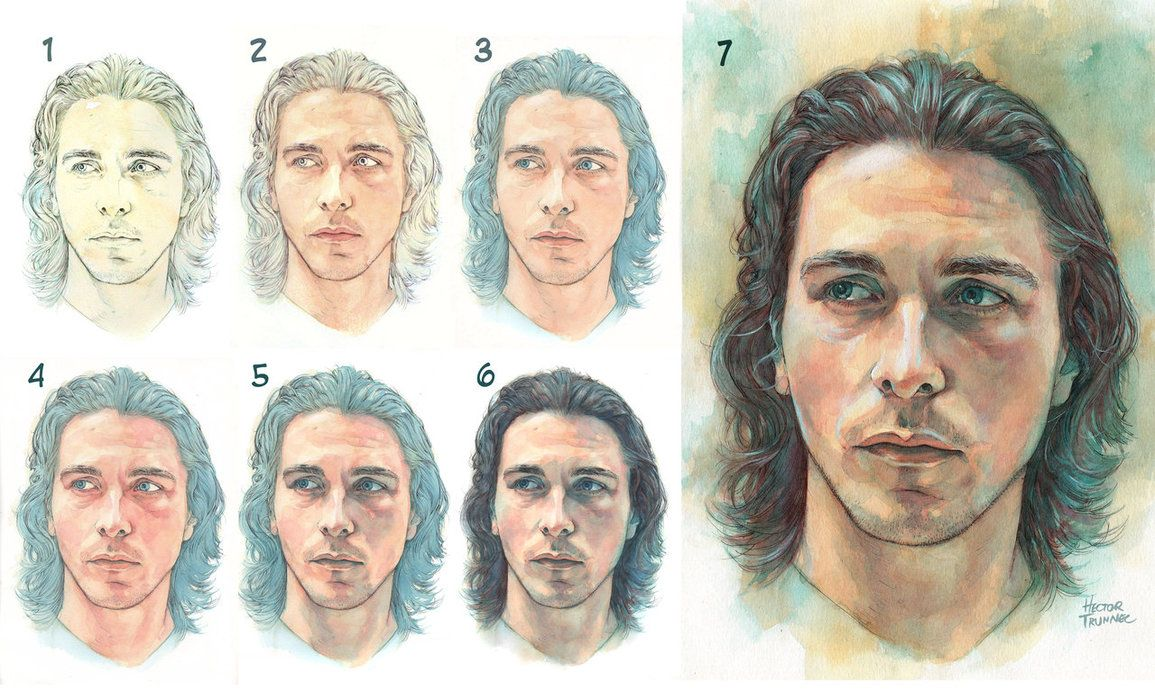
\includegraphics[width=3.64583in,height=3.64583in]{../000_images/004_visualization_step_by_step.jpg}

}

\caption{\label{fig-r-visualization-step-by-step}Analogy of data
visualization as painting step by step (Watercolor portrait - Step by
Step by Hector Trunnec (Valencia, Spain) 2015-03-03)}

\end{figure}%
\end{frame}

\begin{frame}[fragile]{}
\phantomsection\label{section-11}
\begin{itemize}
\tightlist
\item
  \textbf{Histograms: the base R way}
\end{itemize}

\tiny

\begin{Shaded}
\begin{Highlighting}[]
\NormalTok{weekly\_store}\SpecialCharTok{$}\NormalTok{p1sales }\SpecialCharTok{|\textgreater{}} \FunctionTok{hist}\NormalTok{()}
\end{Highlighting}
\end{Shaded}

\begin{center}
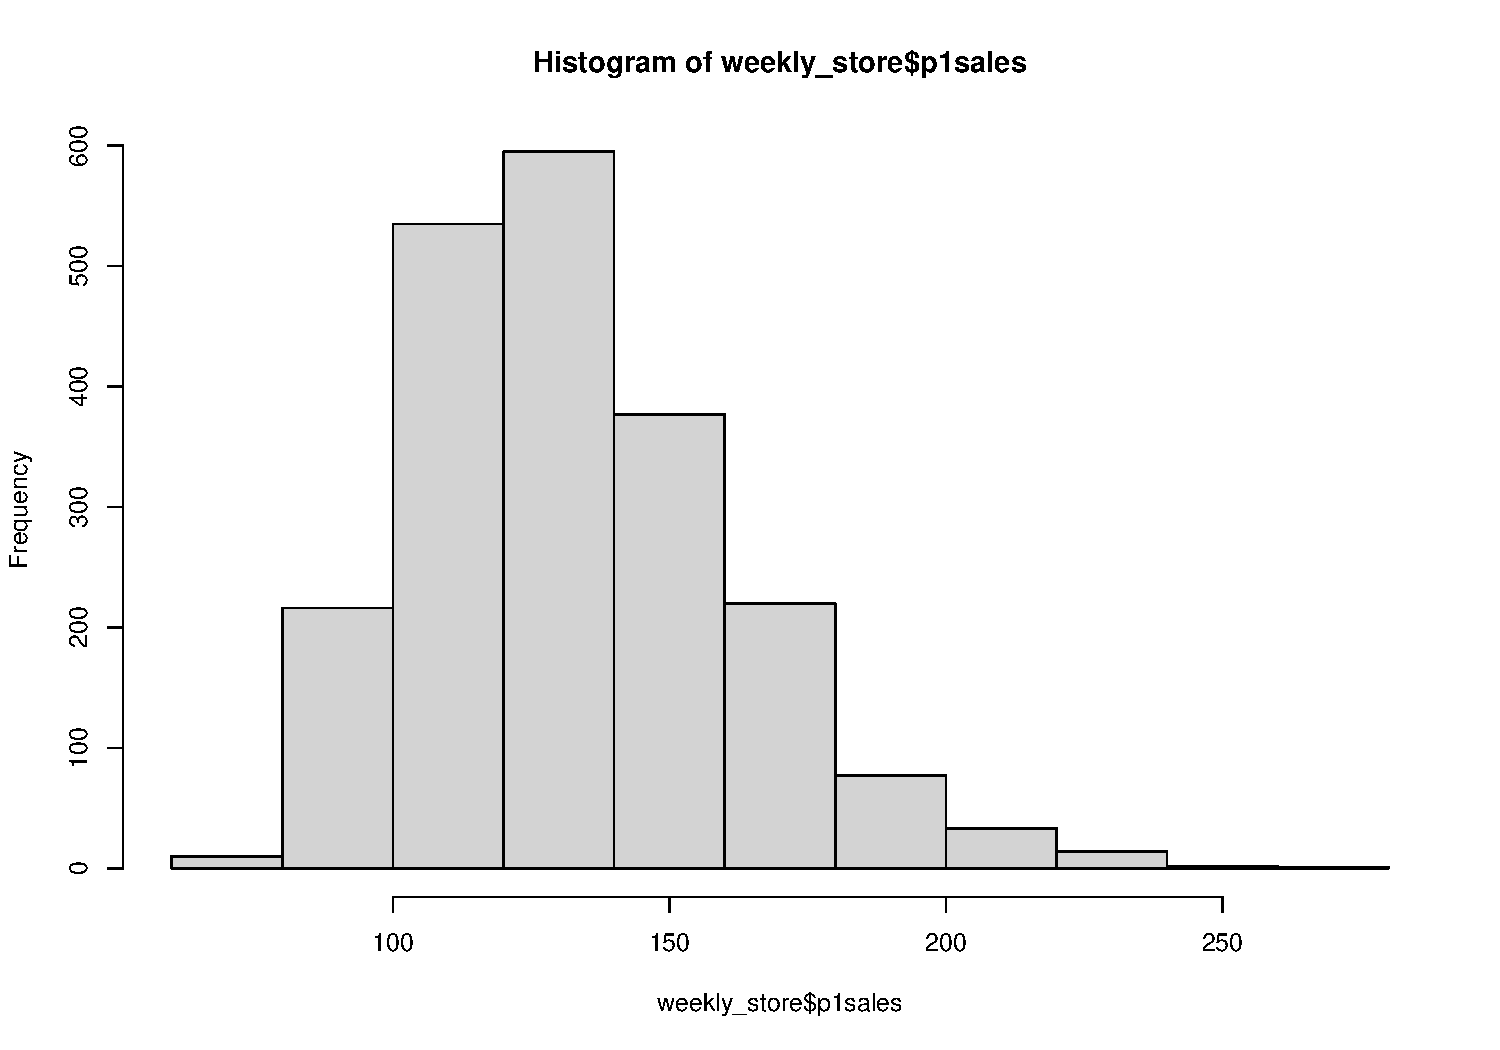
\includegraphics[width=0.5\textwidth,height=\textheight]{003_describing_data_files/figure-beamer/unnamed-chunk-10-1.pdf}
\end{center}
\end{frame}

\begin{frame}[fragile]{}
\phantomsection\label{section-12}
\begin{itemize}
\tightlist
\item
  \textbf{Histograms: the base R way}
\end{itemize}

\tiny

\begin{Shaded}
\begin{Highlighting}[]
\NormalTok{weekly\_store}\SpecialCharTok{$}\NormalTok{p1sales }\SpecialCharTok{|\textgreater{}} \FunctionTok{hist}\NormalTok{(}\AttributeTok{main =} \StringTok{"Product 1 Weekly Sales Frequencies, All Stores"}\NormalTok{,}
                             \AttributeTok{xlab =} \StringTok{"Product1 Sales (Units)"}\NormalTok{ ,}
                             \AttributeTok{ylab =} \StringTok{"Count"}\NormalTok{)}
\end{Highlighting}
\end{Shaded}

\begin{center}
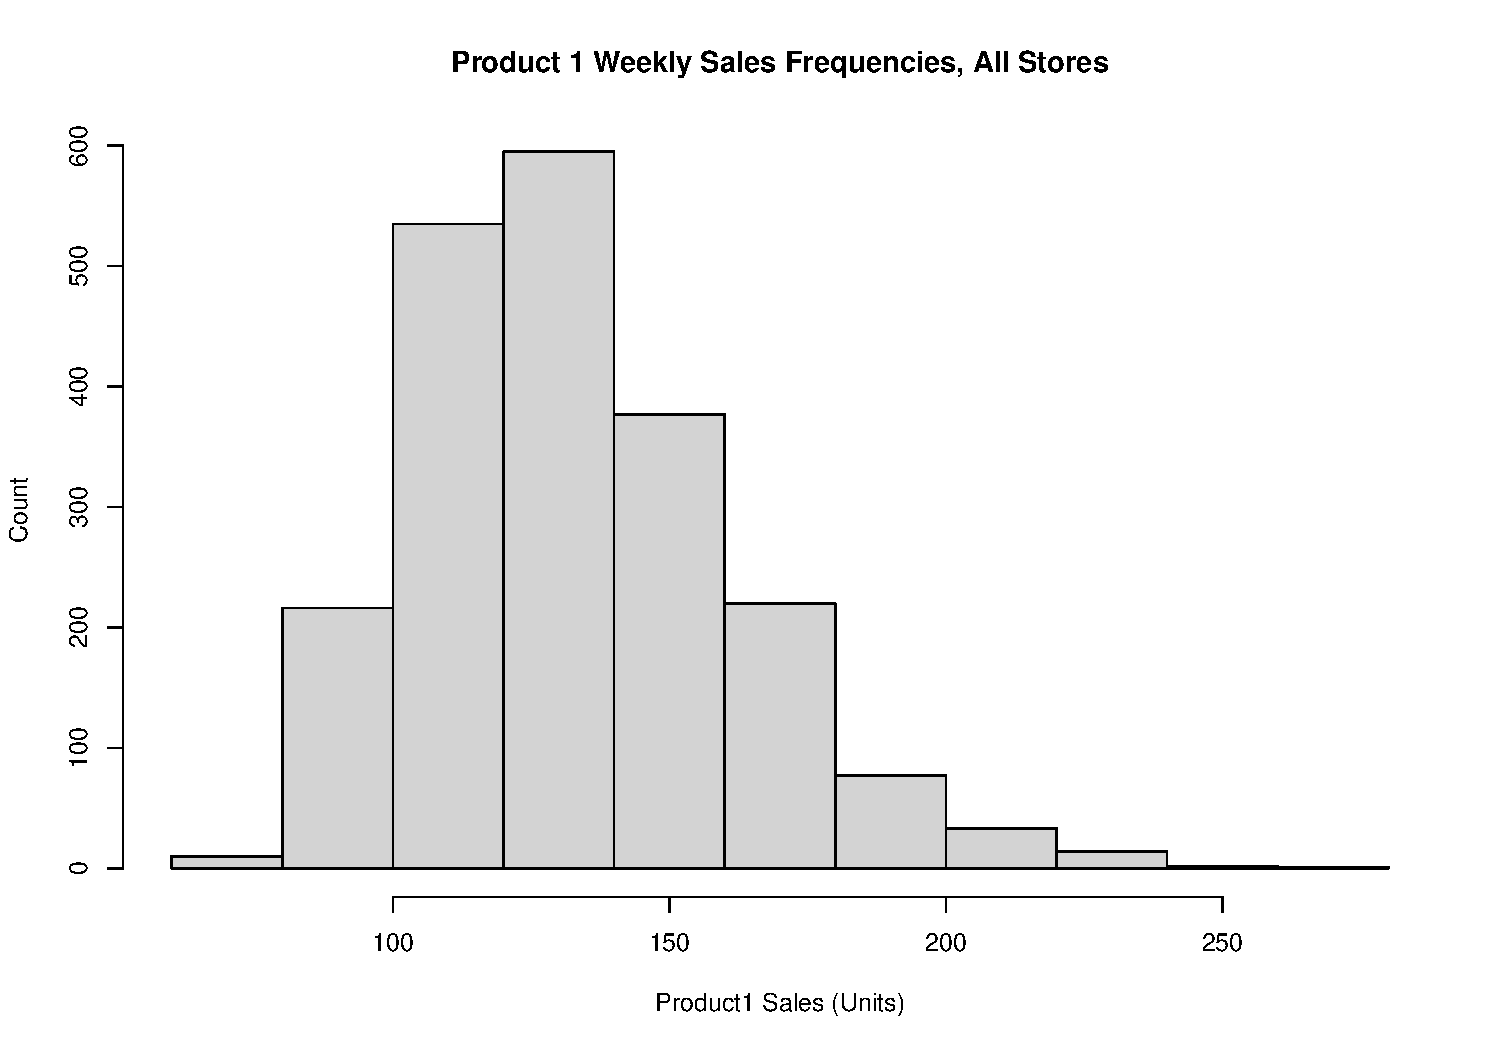
\includegraphics[width=0.5\textwidth,height=\textheight]{003_describing_data_files/figure-beamer/unnamed-chunk-11-1.pdf}
\end{center}
\end{frame}

\begin{frame}[fragile]{}
\phantomsection\label{section-13}
\begin{itemize}
\tightlist
\item
  \textbf{Histograms: the base R way}
\end{itemize}

\tiny

\begin{Shaded}
\begin{Highlighting}[]
\NormalTok{weekly\_store}\SpecialCharTok{$}\NormalTok{p1sales }\SpecialCharTok{|\textgreater{}} \FunctionTok{hist}\NormalTok{(}\AttributeTok{main =} \StringTok{"Product 1 Weekly Sales Frequencies, All Stores"}\NormalTok{,}
                             \AttributeTok{xlab =} \StringTok{"Product1 Sales (Units)"}\NormalTok{ ,}
                             \AttributeTok{ylab =} \StringTok{"Count"}\NormalTok{, }
                             \AttributeTok{breaks =} \DecValTok{30}\NormalTok{, }
                             \AttributeTok{col =}  \StringTok{"lightblue"}\NormalTok{)}
\end{Highlighting}
\end{Shaded}

\begin{center}
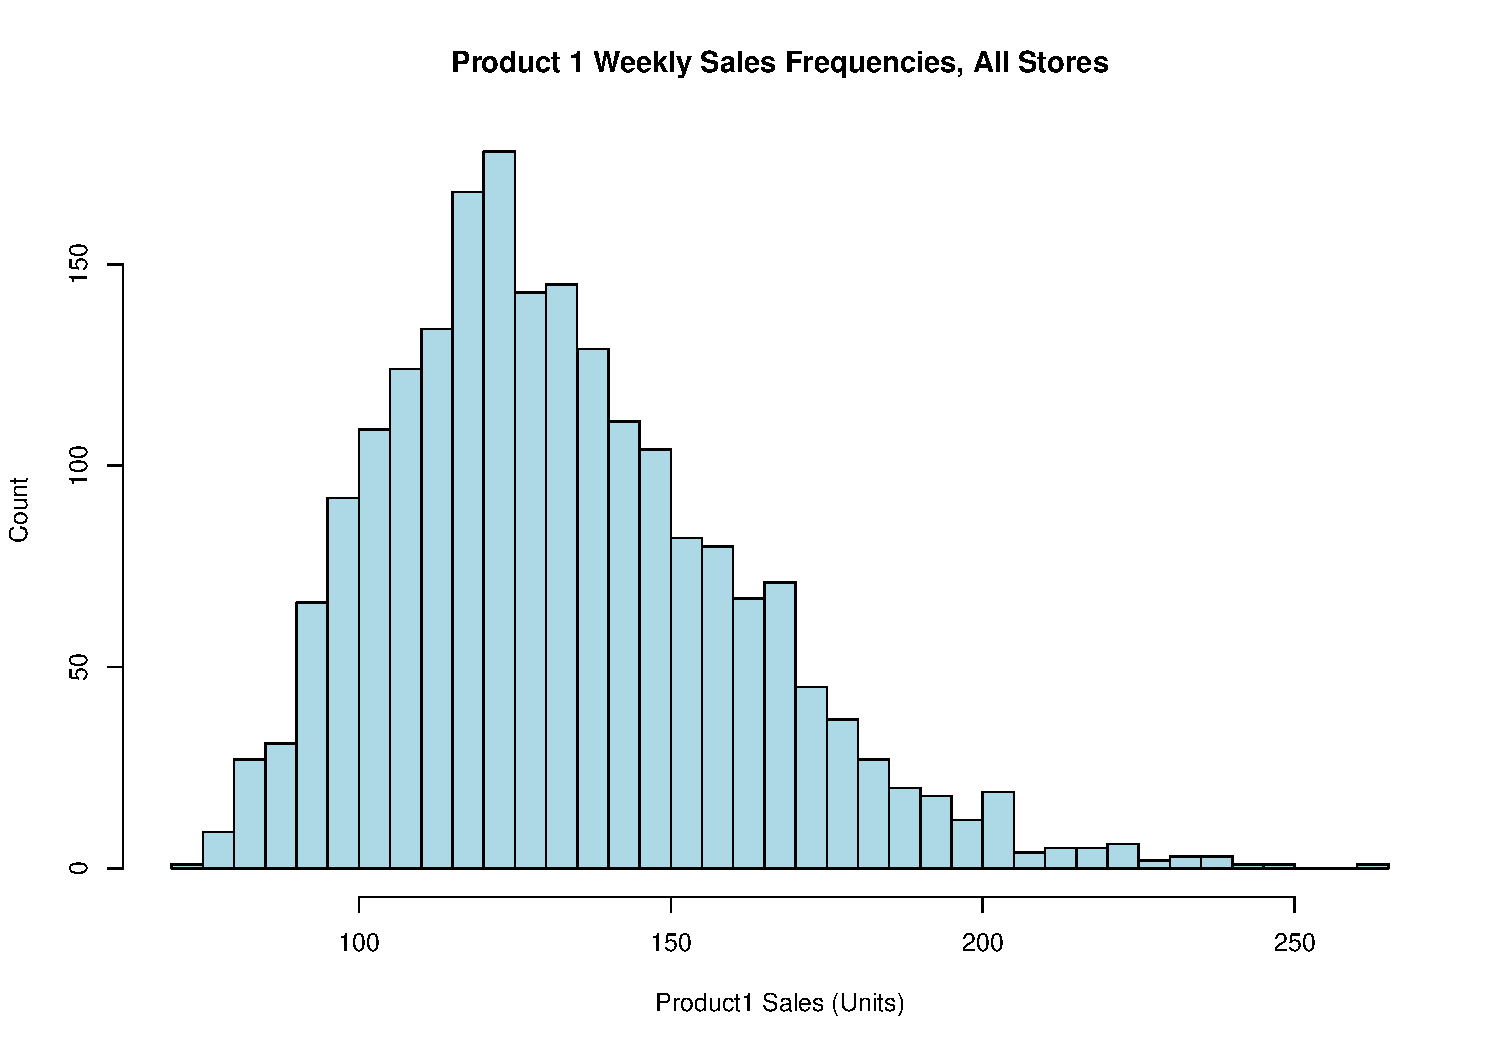
\includegraphics[width=0.5\textwidth,height=\textheight]{003_describing_data_files/figure-beamer/unnamed-chunk-12-1.pdf}
\end{center}
\end{frame}

\begin{frame}[fragile]{}
\phantomsection\label{section-14}
\begin{itemize}
\tightlist
\item
  \textbf{Histograms: the base R way}
\end{itemize}

\tiny

\begin{Shaded}
\begin{Highlighting}[]
\NormalTok{weekly\_store}\SpecialCharTok{$}\NormalTok{p1sales }\SpecialCharTok{|\textgreater{}} \FunctionTok{hist}\NormalTok{(}\AttributeTok{main =} \StringTok{"Product 1 Weekly Sales Frequencies, All Stores"}\NormalTok{,}
                             \AttributeTok{xlab =} \StringTok{"Product1 Sales (Units)"}\NormalTok{ ,}
                             \AttributeTok{ylab =} \StringTok{"Frequency"}\NormalTok{, }
                             \AttributeTok{breaks =} \DecValTok{30}\NormalTok{, }
                             \AttributeTok{col =}  \StringTok{"lightblue"}\NormalTok{, }
                             \AttributeTok{freq =} \ConstantTok{FALSE}\NormalTok{,}
                             \AttributeTok{xaxt =} \StringTok{"n"}\NormalTok{)}
\end{Highlighting}
\end{Shaded}

\begin{center}
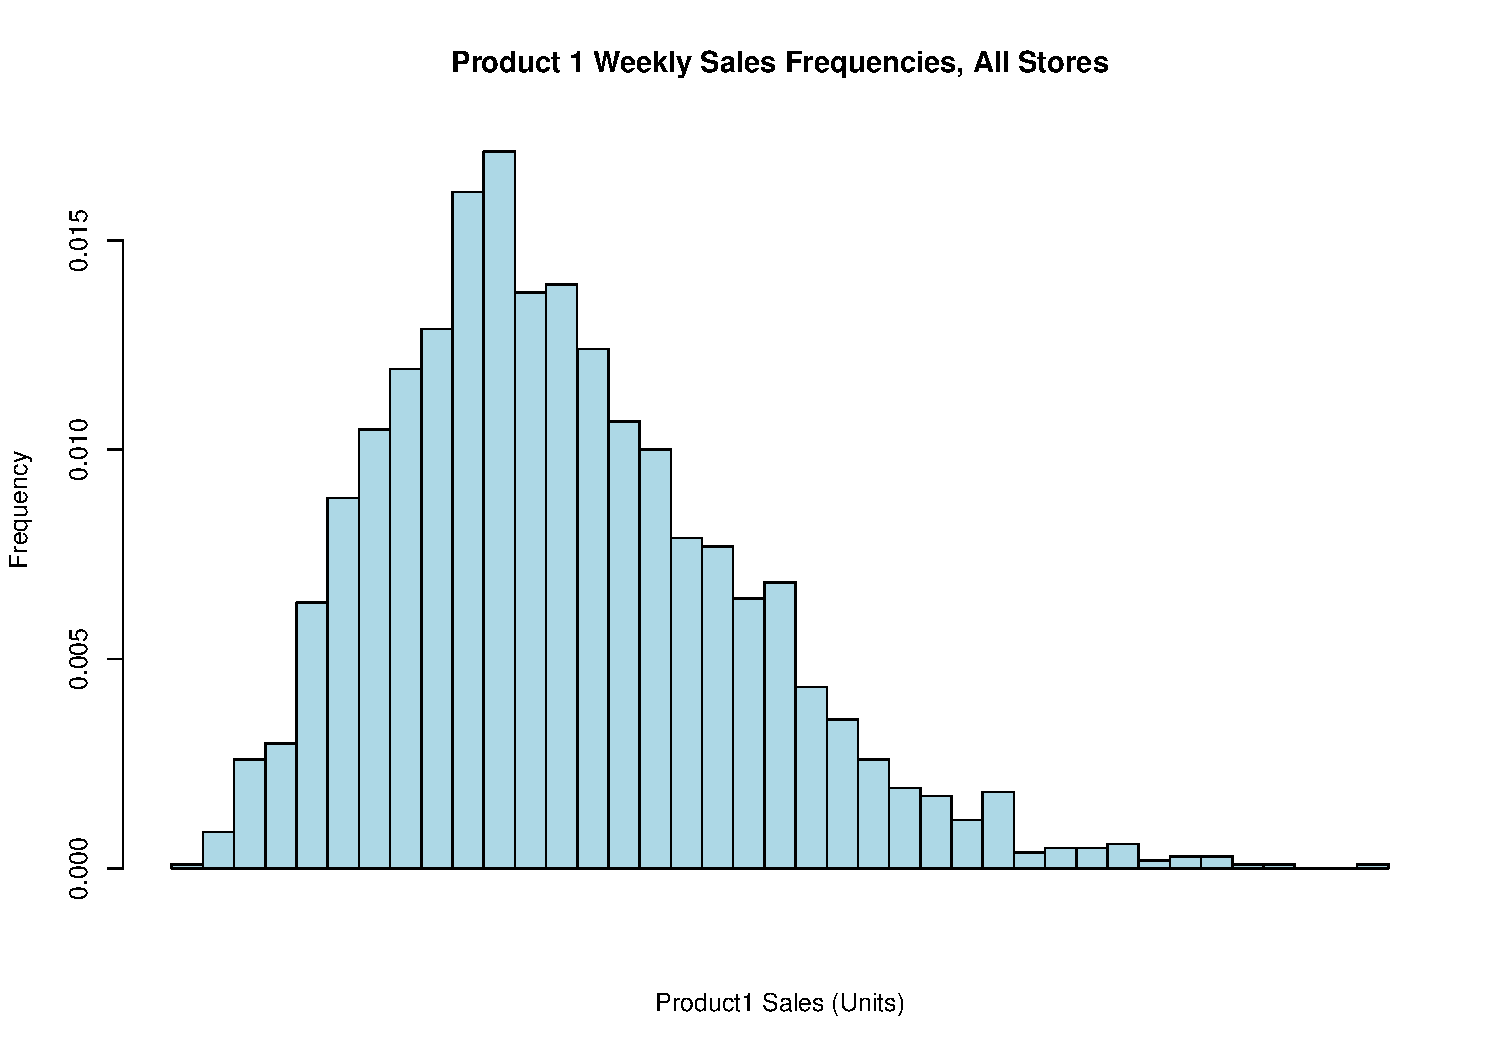
\includegraphics[width=0.5\textwidth,height=\textheight]{003_describing_data_files/figure-beamer/unnamed-chunk-13-1.pdf}
\end{center}
\end{frame}

\begin{frame}[fragile]{}
\phantomsection\label{section-15}
\begin{itemize}
\tightlist
\item
  \textbf{Histograms: the base R way}
\end{itemize}

\tiny

\begin{Shaded}
\begin{Highlighting}[]
\NormalTok{weekly\_store}\SpecialCharTok{$}\NormalTok{p1sales }\SpecialCharTok{|\textgreater{}} \FunctionTok{hist}\NormalTok{(}\AttributeTok{main =} \StringTok{"Product 1 Weekly Sales Frequencies, All Stores"}\NormalTok{,}
                             \AttributeTok{xlab =} \StringTok{"Product1 Sales (Units)"}\NormalTok{ ,}
                             \AttributeTok{ylab =} \StringTok{"Frequency"}\NormalTok{, }
                             \AttributeTok{breaks =} \DecValTok{30}\NormalTok{, }
                             \AttributeTok{col =}  \StringTok{"lightblue"}\NormalTok{, }
                             \AttributeTok{freq =} \ConstantTok{FALSE}\NormalTok{,}
                             \AttributeTok{xaxt =} \StringTok{"n"}\NormalTok{)}
\FunctionTok{axis}\NormalTok{(}\AttributeTok{side=}\DecValTok{1}\NormalTok{ , }\AttributeTok{at=}\FunctionTok{seq}\NormalTok{(}\AttributeTok{from =} \DecValTok{60}\NormalTok{, }\AttributeTok{to =} \DecValTok{300}\NormalTok{, }\AttributeTok{by =} \DecValTok{20}\NormalTok{))}
\end{Highlighting}
\end{Shaded}

\begin{center}
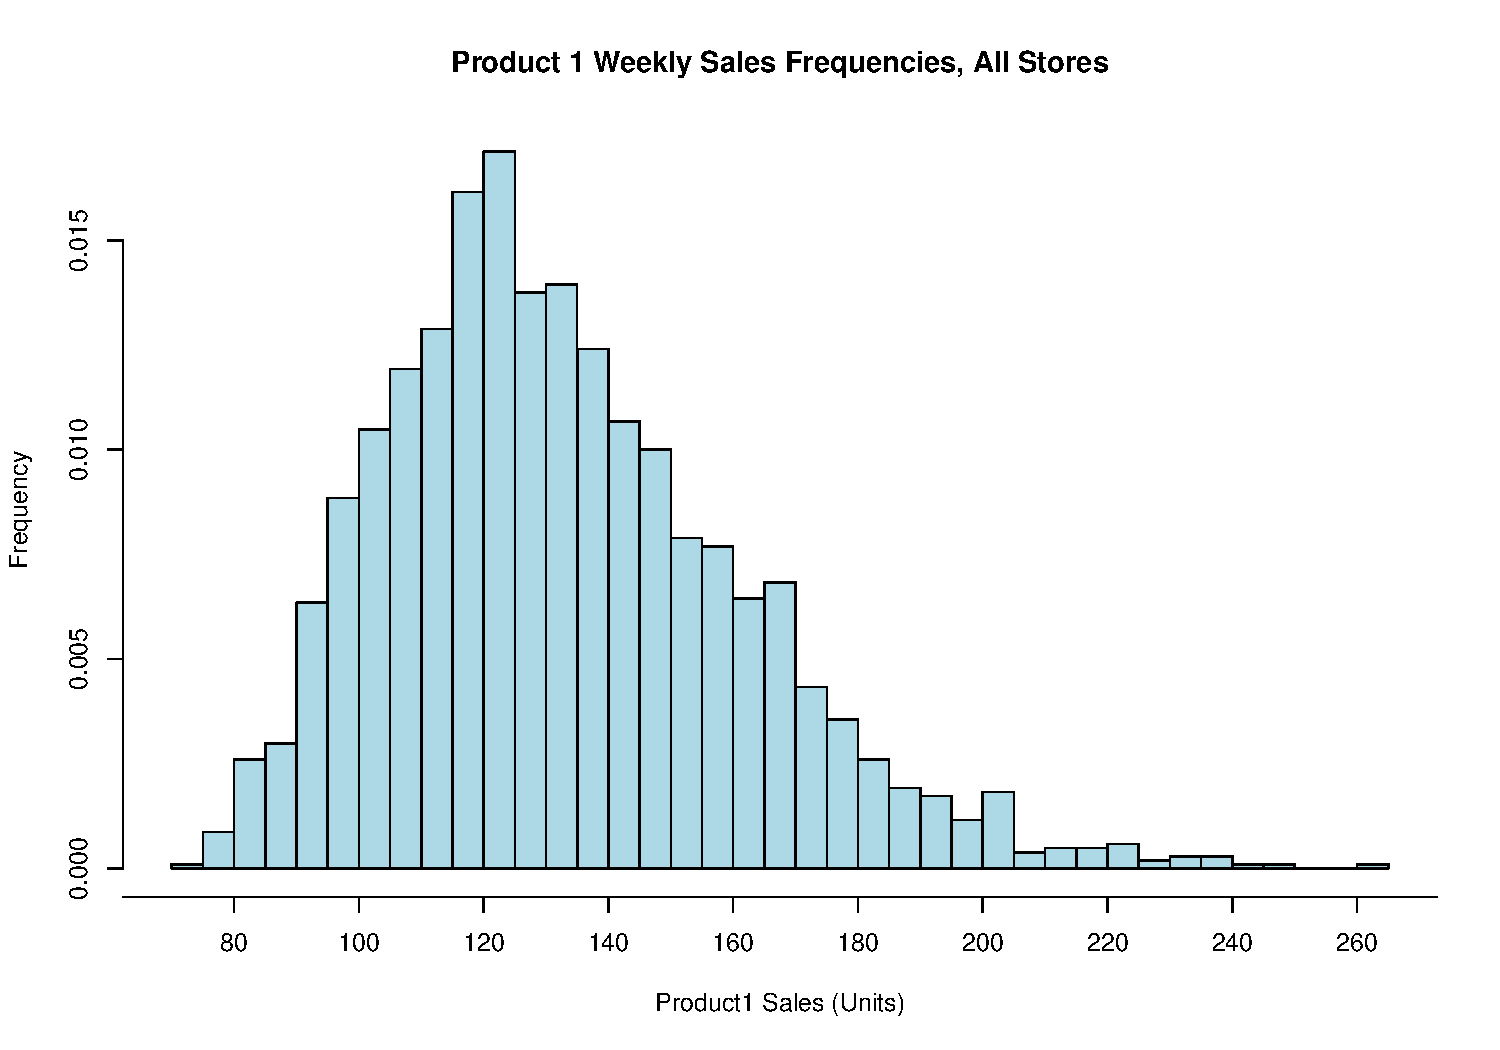
\includegraphics[width=0.5\textwidth,height=\textheight]{003_describing_data_files/figure-beamer/unnamed-chunk-14-1.pdf}
\end{center}
\end{frame}

\begin{frame}[fragile]{}
\phantomsection\label{section-16}
\begin{itemize}
\tightlist
\item
  \textbf{Histograms: the base R way}
\end{itemize}

\tiny

\begin{Shaded}
\begin{Highlighting}[]
\NormalTok{weekly\_store}\SpecialCharTok{$}\NormalTok{p1sales }\SpecialCharTok{|\textgreater{}} \FunctionTok{hist}\NormalTok{(}\AttributeTok{main =} \StringTok{"Product 1 Weekly Sales Frequencies, All Stores"}\NormalTok{,}
                             \AttributeTok{xlab =} \StringTok{"Product1 Sales (Units)"}\NormalTok{ ,}
                             \AttributeTok{ylab =} \StringTok{"Frequency"}\NormalTok{, }
                             \AttributeTok{breaks =} \DecValTok{30}\NormalTok{, }
                             \AttributeTok{col =}  \StringTok{"lightblue"}\NormalTok{, }
                             \AttributeTok{freq =} \ConstantTok{FALSE}\NormalTok{,}
                             \AttributeTok{xaxt =} \StringTok{"n"}\NormalTok{)}
\FunctionTok{axis}\NormalTok{(}\AttributeTok{side=}\DecValTok{1}\NormalTok{ , }\AttributeTok{at=}\FunctionTok{seq}\NormalTok{(}\AttributeTok{from =} \DecValTok{60}\NormalTok{, }\AttributeTok{to =} \DecValTok{300}\NormalTok{, }\AttributeTok{by =} \DecValTok{20}\NormalTok{))}
\FunctionTok{lines}\NormalTok{(}\AttributeTok{x =} \FunctionTok{density}\NormalTok{(weekly\_store}\SpecialCharTok{$}\NormalTok{p1sales, }\AttributeTok{bw=}\DecValTok{10}\NormalTok{), }\AttributeTok{type=}\StringTok{"l"}\NormalTok{, }\AttributeTok{col=}\StringTok{"darkred"}\NormalTok{, }\AttributeTok{lwd=}\DecValTok{2}\NormalTok{)}
\end{Highlighting}
\end{Shaded}

\begin{center}
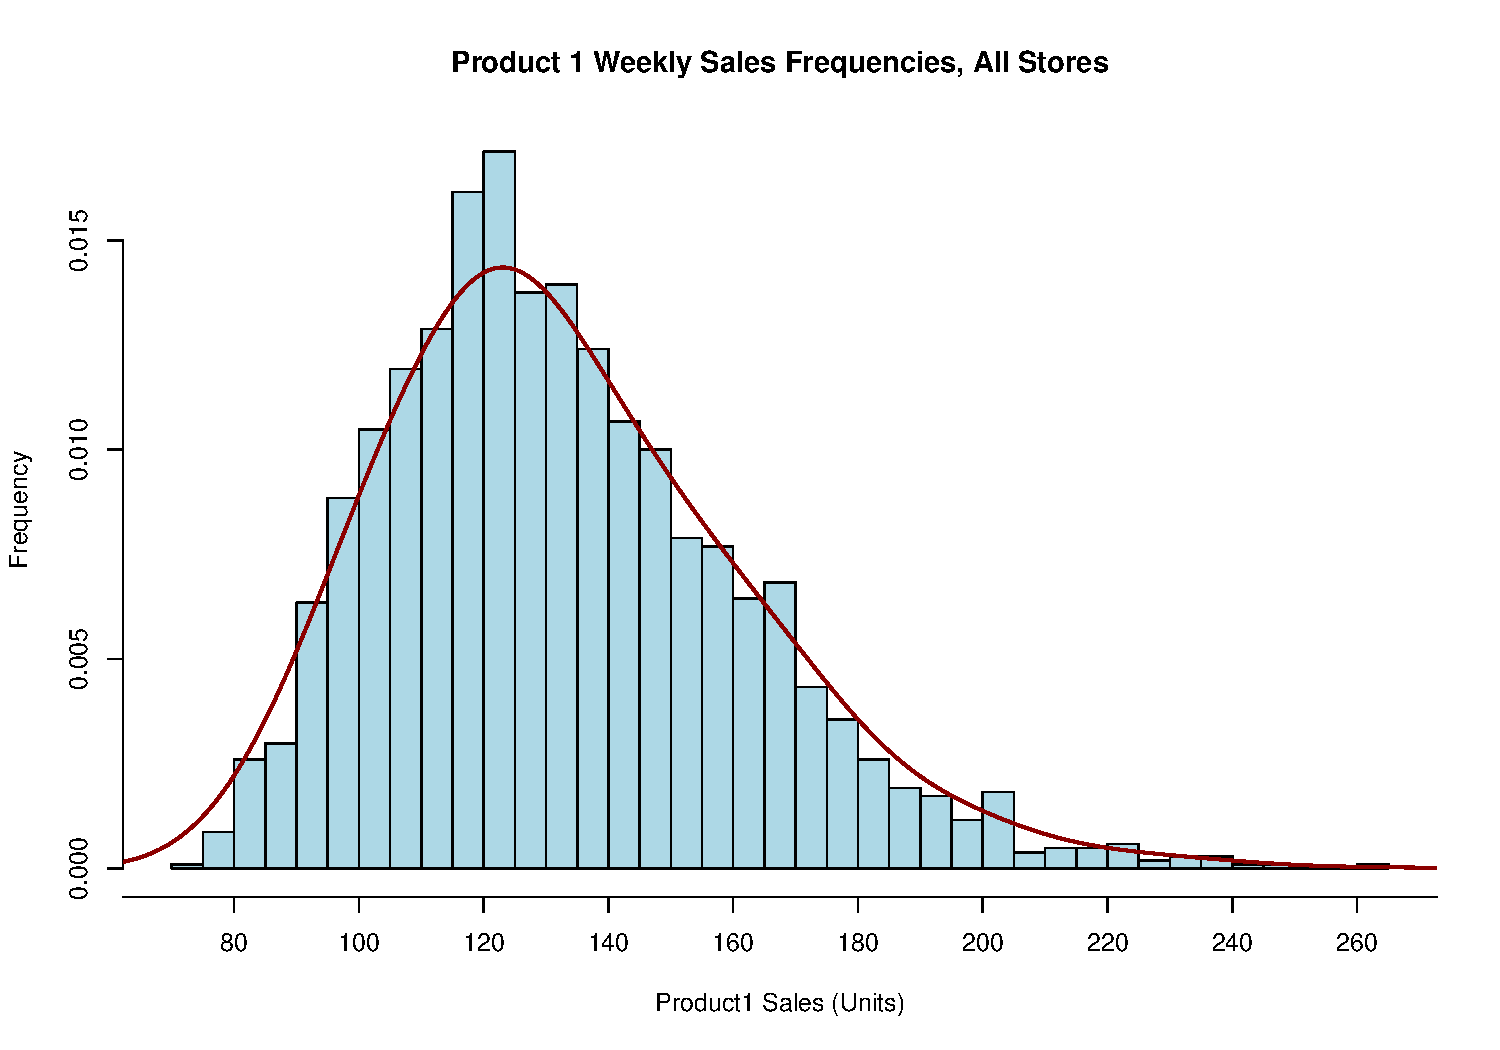
\includegraphics[width=0.5\textwidth,height=\textheight]{003_describing_data_files/figure-beamer/unnamed-chunk-15-1.pdf}
\end{center}
\end{frame}

\begin{frame}[fragile]{}
\phantomsection\label{section-17}
\begin{itemize}
\tightlist
\item
  \textbf{Histograms: the tidyverse way}
\end{itemize}

\tiny

\begin{Shaded}
\begin{Highlighting}[]
\NormalTok{weekly\_store }\SpecialCharTok{|\textgreater{}} \FunctionTok{ggplot}\NormalTok{()}
\end{Highlighting}
\end{Shaded}

\begin{center}

\includegraphics[width=0.5\textwidth,height=\textheight]{003_describing_data_files/figure-beamer/unnamed-chunk-16-1.pdf}
\end{center}
\end{frame}

\begin{frame}[fragile]{}
\phantomsection\label{section-18}
\begin{itemize}
\tightlist
\item
  \textbf{Histograms: the tidyverse way}
\end{itemize}

\tiny

\begin{Shaded}
\begin{Highlighting}[]
\NormalTok{weekly\_store }\SpecialCharTok{|\textgreater{}} \FunctionTok{ggplot}\NormalTok{() }\SpecialCharTok{+} 
  \FunctionTok{geom\_histogram}\NormalTok{(}\FunctionTok{aes}\NormalTok{(}\AttributeTok{x =}\NormalTok{ p1sales, }\AttributeTok{y =} \FunctionTok{after\_stat}\NormalTok{(density)),}
                 \AttributeTok{color =} \StringTok{"black"}\NormalTok{, }\AttributeTok{fill =} \StringTok{"lightblue"}\NormalTok{, }\AttributeTok{bins =} \DecValTok{30}\NormalTok{)}
\end{Highlighting}
\end{Shaded}

\begin{center}
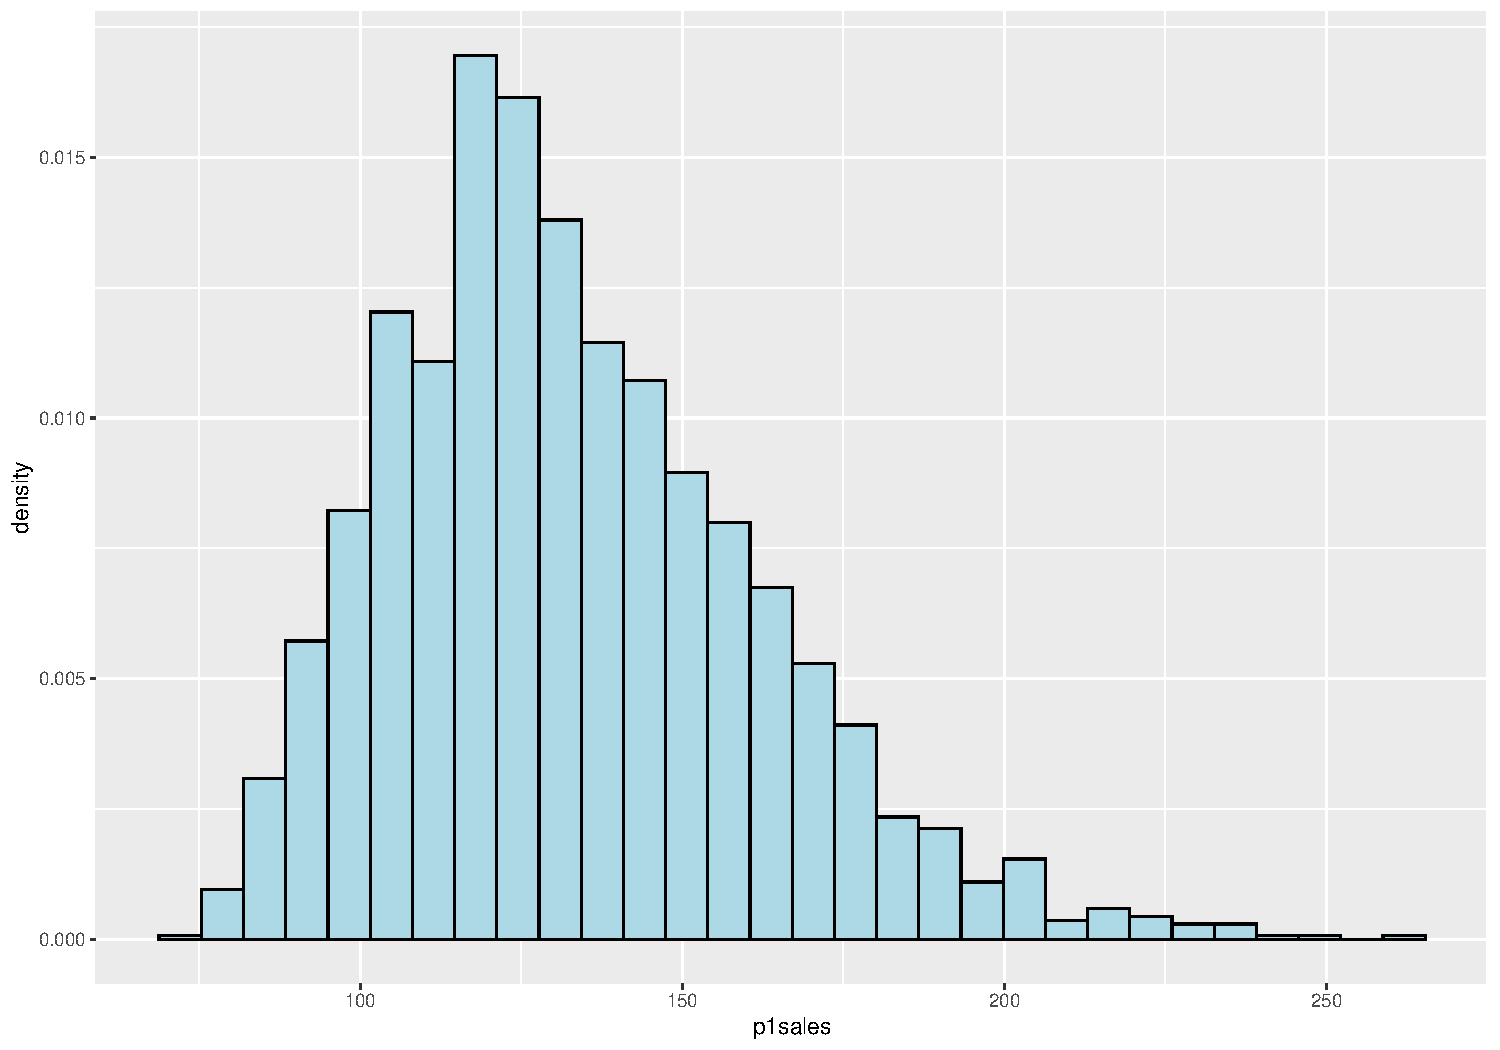
\includegraphics[width=0.5\textwidth,height=\textheight]{003_describing_data_files/figure-beamer/unnamed-chunk-17-1.pdf}
\end{center}
\end{frame}

\begin{frame}[fragile]{}
\phantomsection\label{section-19}
\begin{itemize}
\tightlist
\item
  \textbf{Histograms: the tidyverse way}
\end{itemize}

\tiny

\begin{Shaded}
\begin{Highlighting}[]
\NormalTok{weekly\_store }\SpecialCharTok{|\textgreater{}} \FunctionTok{ggplot}\NormalTok{() }\SpecialCharTok{+} 
  \FunctionTok{geom\_histogram}\NormalTok{(}\FunctionTok{aes}\NormalTok{(}\AttributeTok{x =}\NormalTok{ p1sales, }\AttributeTok{y =} \FunctionTok{after\_stat}\NormalTok{(density)),}
                 \AttributeTok{color =} \StringTok{"black"}\NormalTok{, }\AttributeTok{fill =} \StringTok{"lightblue"}\NormalTok{, }\AttributeTok{bins =} \DecValTok{30}\NormalTok{) }\SpecialCharTok{+}
  \FunctionTok{geom\_density}\NormalTok{(}\FunctionTok{aes}\NormalTok{(}\AttributeTok{x=}\NormalTok{p1sales),}
               \AttributeTok{bw=}\DecValTok{10}\NormalTok{, }\AttributeTok{color=}\StringTok{"darkred"}\NormalTok{,}
               \AttributeTok{linetype =} \StringTok{"solid"}\NormalTok{, }\AttributeTok{linewidth =} \DecValTok{1}\NormalTok{)}
\end{Highlighting}
\end{Shaded}

\begin{center}
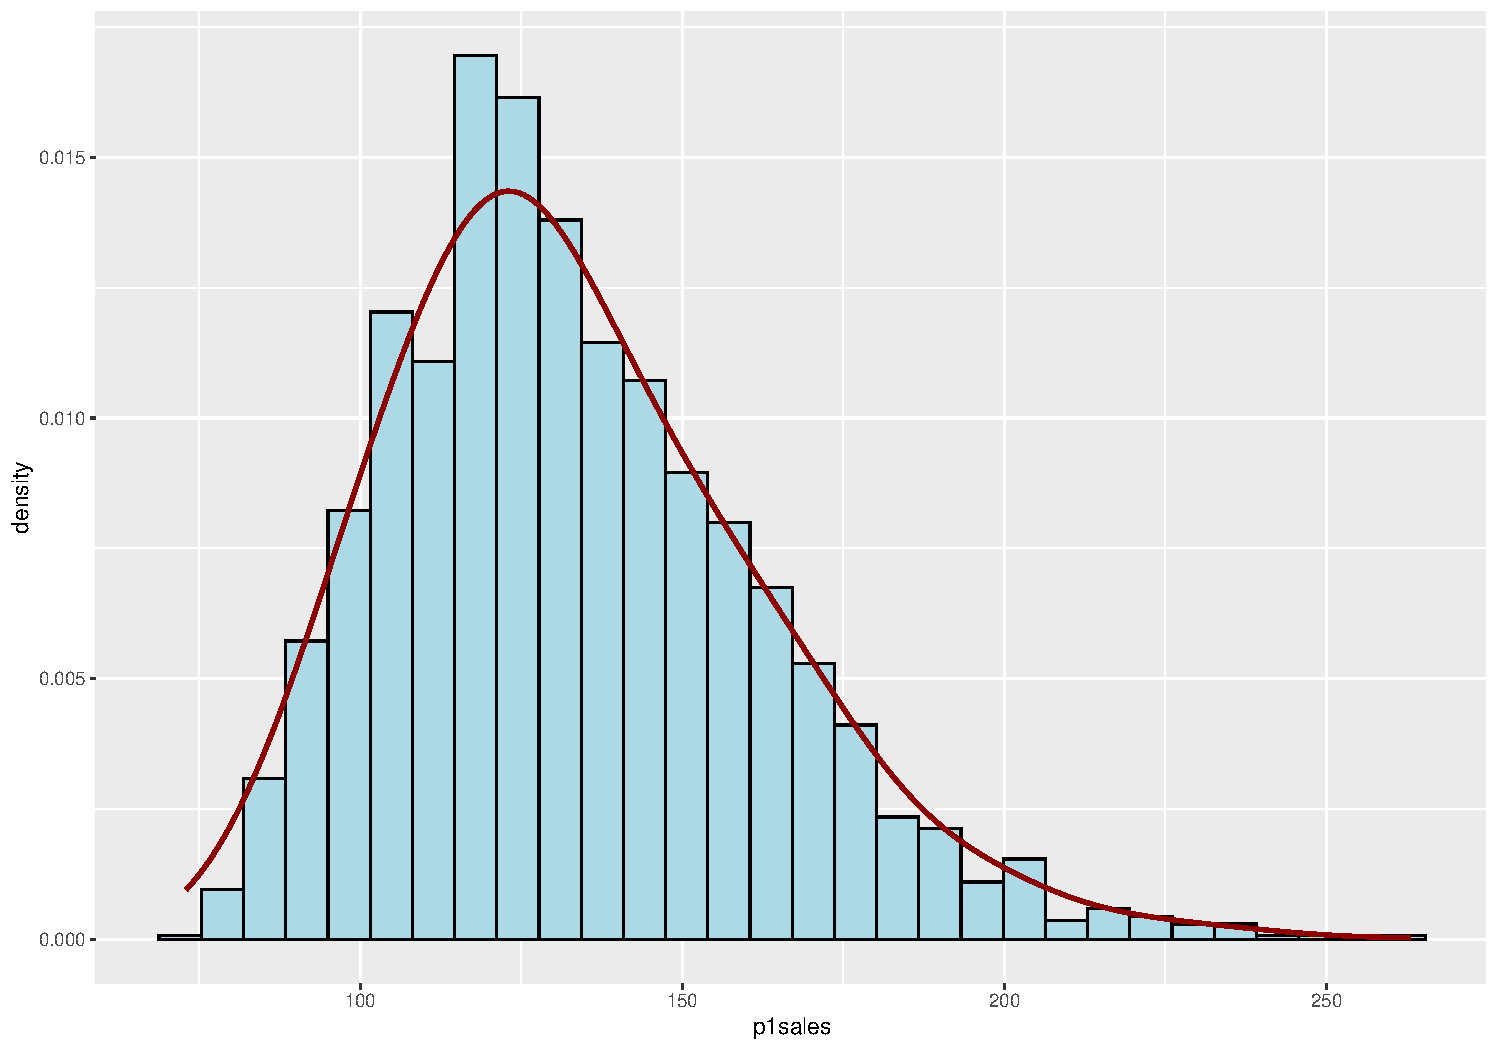
\includegraphics[width=0.5\textwidth,height=\textheight]{003_describing_data_files/figure-beamer/unnamed-chunk-18-1.pdf}
\end{center}
\end{frame}

\begin{frame}[fragile]{}
\phantomsection\label{section-20}
\begin{itemize}
\tightlist
\item
  \textbf{Histograms: the tidyverse way}
\end{itemize}

\tiny

\begin{Shaded}
\begin{Highlighting}[]
\NormalTok{weekly\_store }\SpecialCharTok{|\textgreater{}} \FunctionTok{ggplot}\NormalTok{() }\SpecialCharTok{+} 
  \FunctionTok{geom\_histogram}\NormalTok{(}\FunctionTok{aes}\NormalTok{(}\AttributeTok{x=}\NormalTok{p1sales, }\AttributeTok{y =} \FunctionTok{after\_stat}\NormalTok{(density)),}
                 \AttributeTok{color =} \StringTok{"black"}\NormalTok{, }\AttributeTok{fill =} \StringTok{"lightblue"}\NormalTok{, }\AttributeTok{bins =} \DecValTok{30}\NormalTok{) }\SpecialCharTok{+}
  \FunctionTok{geom\_density}\NormalTok{(}\FunctionTok{aes}\NormalTok{(}\AttributeTok{x=}\NormalTok{p1sales),}
               \AttributeTok{bw=}\DecValTok{10}\NormalTok{, }\AttributeTok{color=}\StringTok{"darkred"}\NormalTok{, }\AttributeTok{linetype=}\StringTok{"solid"}\NormalTok{, }\AttributeTok{linewidth=}\DecValTok{1}\NormalTok{) }\SpecialCharTok{+} 
  \FunctionTok{scale\_x\_continuous}\NormalTok{(}\AttributeTok{breaks =} \FunctionTok{seq}\NormalTok{(}\AttributeTok{from =} \DecValTok{60}\NormalTok{, }\AttributeTok{to =} \DecValTok{300}\NormalTok{, }\AttributeTok{by =} \DecValTok{20}\NormalTok{))}
\end{Highlighting}
\end{Shaded}

\begin{center}
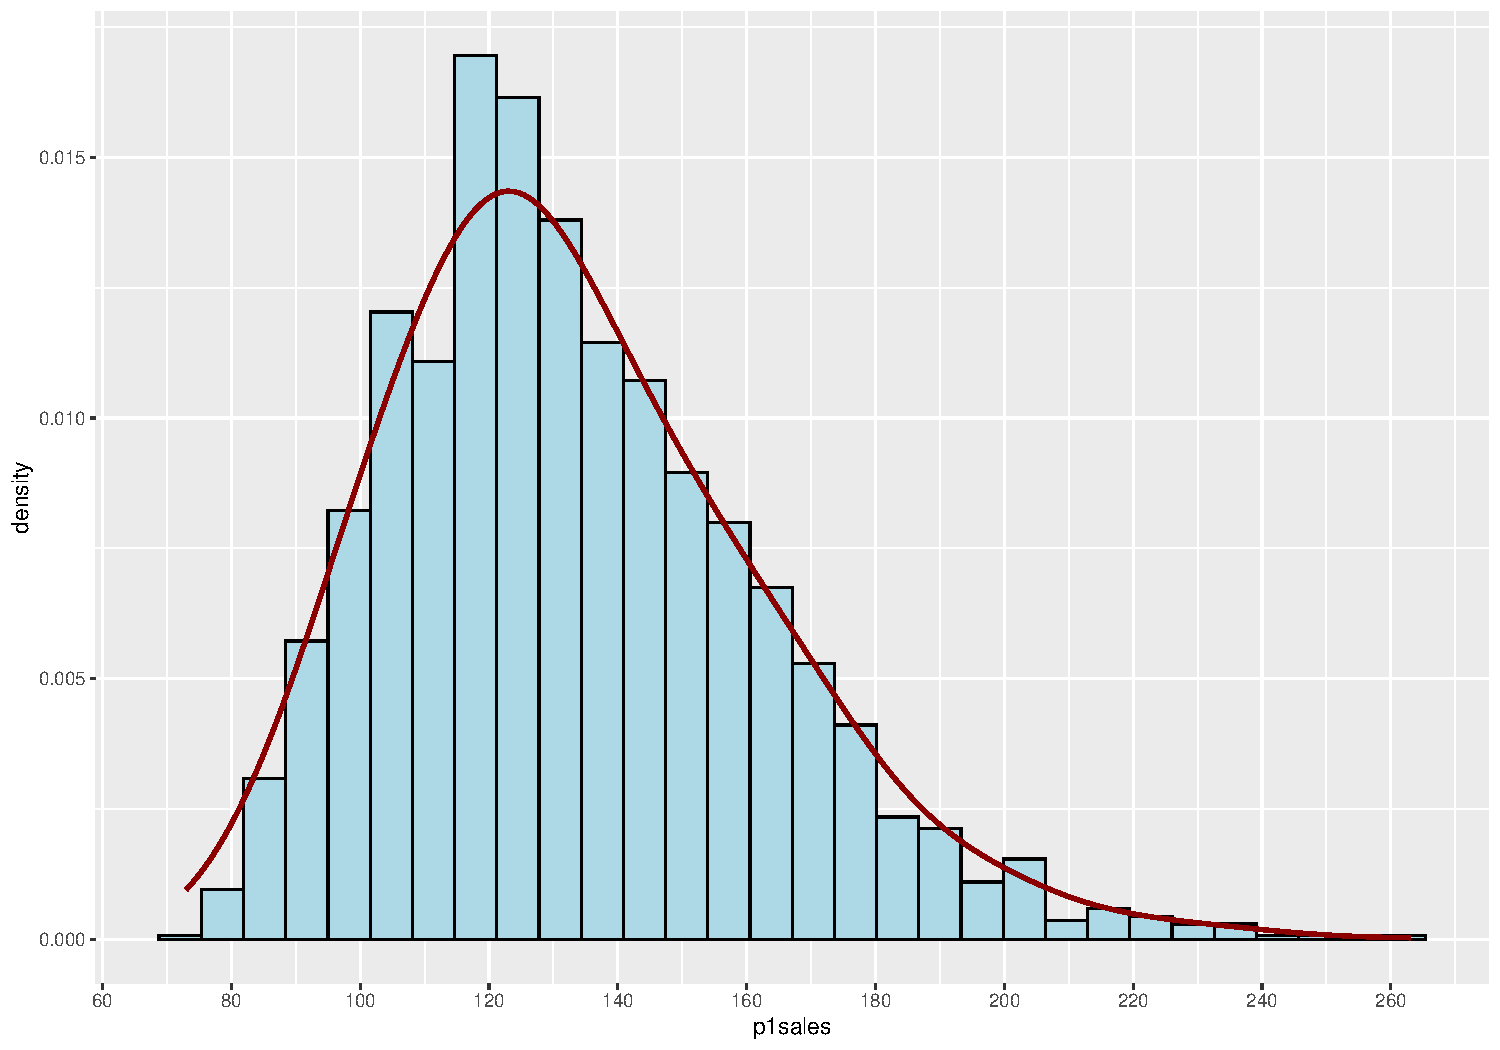
\includegraphics[width=0.5\textwidth,height=\textheight]{003_describing_data_files/figure-beamer/unnamed-chunk-19-1.pdf}
\end{center}
\end{frame}

\begin{frame}[fragile]{}
\phantomsection\label{section-21}
\begin{itemize}
\tightlist
\item
  \textbf{Histograms: the tidyverse way}
\end{itemize}

\tiny

\begin{Shaded}
\begin{Highlighting}[]
\NormalTok{weekly\_store }\SpecialCharTok{|\textgreater{}} \FunctionTok{ggplot}\NormalTok{() }\SpecialCharTok{+} 
  \FunctionTok{geom\_histogram}\NormalTok{(}\FunctionTok{aes}\NormalTok{(}\AttributeTok{x =}\NormalTok{ p1sales, }\AttributeTok{y =} \FunctionTok{after\_stat}\NormalTok{(density)),}
                 \AttributeTok{color =} \StringTok{"black"}\NormalTok{, }\AttributeTok{fill =} \StringTok{"lightblue"}\NormalTok{, }\AttributeTok{bins =} \DecValTok{30}\NormalTok{) }\SpecialCharTok{+}
  \FunctionTok{geom\_density}\NormalTok{(}\FunctionTok{aes}\NormalTok{(}\AttributeTok{x =}\NormalTok{ p1sales),}
               \AttributeTok{bw =} \DecValTok{10}\NormalTok{, }\AttributeTok{color =} \StringTok{"darkred"}\NormalTok{, }\AttributeTok{linetype =} \StringTok{"solid"}\NormalTok{, }\AttributeTok{linewidth =} \DecValTok{1}\NormalTok{) }\SpecialCharTok{+} 
  \FunctionTok{scale\_x\_continuous}\NormalTok{(}\AttributeTok{breaks =} \FunctionTok{seq}\NormalTok{(}\AttributeTok{from =} \DecValTok{60}\NormalTok{, }\AttributeTok{to =} \DecValTok{300}\NormalTok{, }\AttributeTok{by =} \DecValTok{20}\NormalTok{)) }\SpecialCharTok{+}
  \FunctionTok{labs}\NormalTok{(}\AttributeTok{x =} \StringTok{"Product1 Sales (Units)"}\NormalTok{, }\AttributeTok{y =} \StringTok{"Frequency"}\NormalTok{, }
       \AttributeTok{title =} \StringTok{"Product 1 Weekly Sales Frequencies, All Stores"}\NormalTok{)}
\end{Highlighting}
\end{Shaded}

\begin{center}
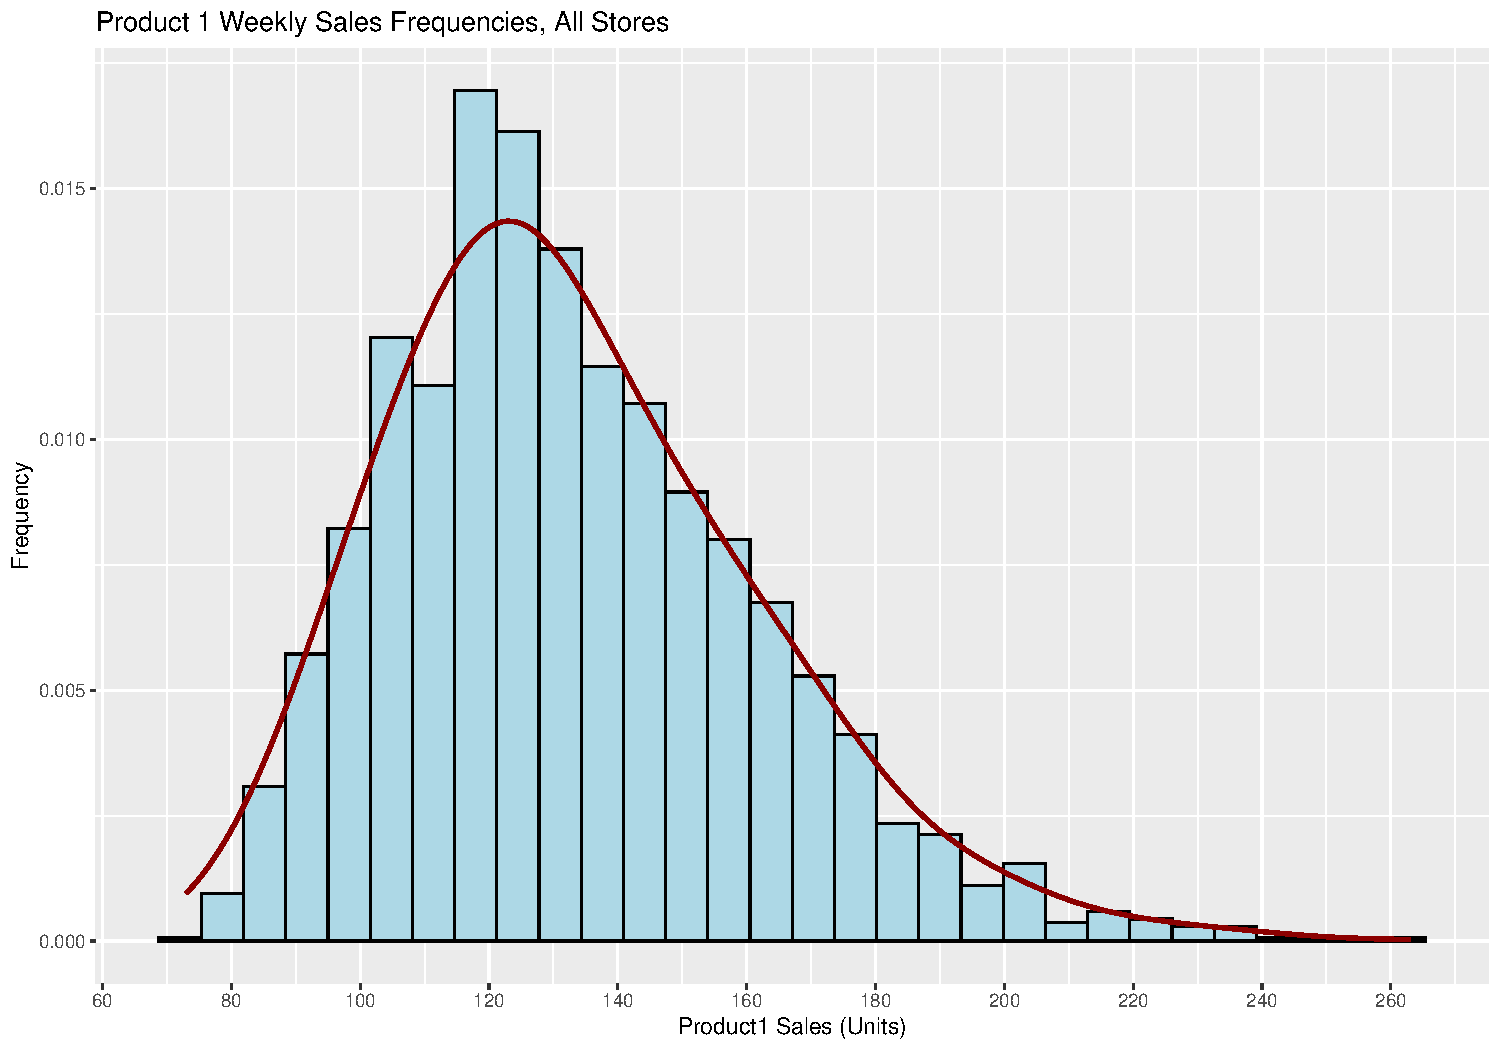
\includegraphics[width=0.5\textwidth,height=\textheight]{003_describing_data_files/figure-beamer/unnamed-chunk-20-1.pdf}
\end{center}
\end{frame}

\begin{frame}[fragile]{}
\phantomsection\label{section-22}
\begin{itemize}
\item
  \textbf{Boxplots: the base R way}

  \begin{itemize}
  \tightlist
  \item
    Boxplot product 2 sales by promotion
  \end{itemize}
\end{itemize}

\tiny

\begin{Shaded}
\begin{Highlighting}[]
\FunctionTok{boxplot}\NormalTok{(weekly\_store}\SpecialCharTok{$}\NormalTok{p2sales }\SpecialCharTok{\textasciitilde{}}\NormalTok{ weekly\_store}\SpecialCharTok{$}\NormalTok{p2prom,}
        \AttributeTok{main =} \StringTok{"Weekly sales of P2 with and without promotion"}\NormalTok{,}
        \AttributeTok{xlab =} \StringTok{"Weekly unit sales"}\NormalTok{, }\AttributeTok{ylab =} \StringTok{"P2 promoted in store?"}\NormalTok{,}
        \AttributeTok{horizontal =} \ConstantTok{TRUE}\NormalTok{, }\AttributeTok{las =} \DecValTok{1}\NormalTok{)}
\end{Highlighting}
\end{Shaded}

\begin{center}
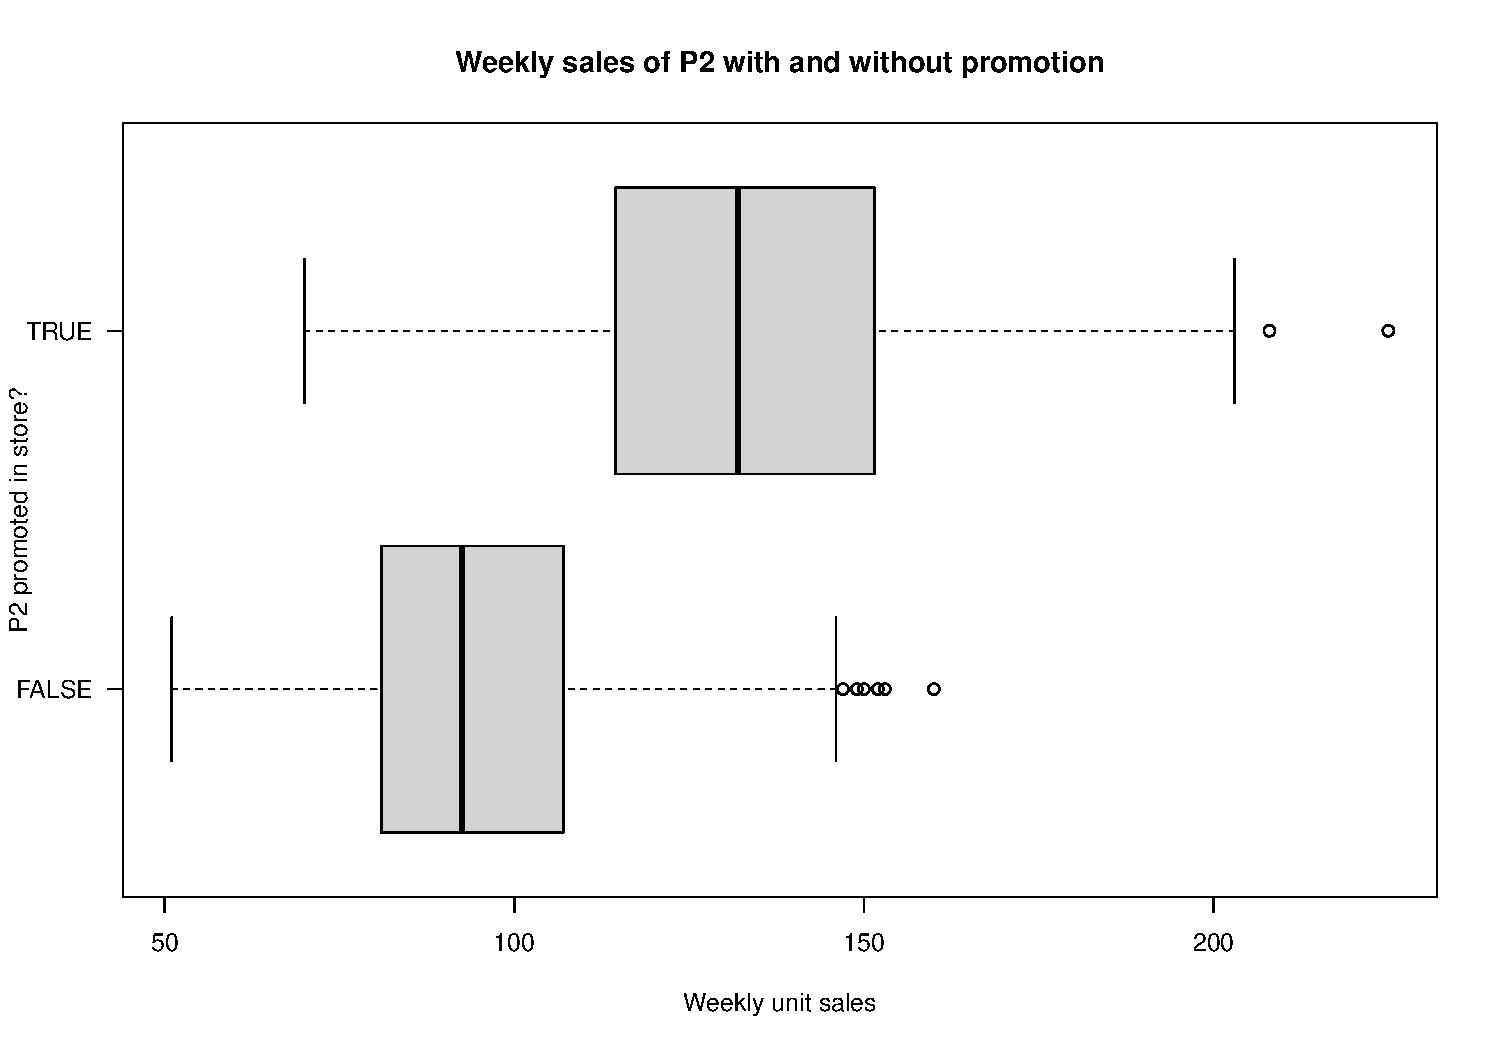
\includegraphics[width=0.5\textwidth,height=\textheight]{003_describing_data_files/figure-beamer/unnamed-chunk-21-1.pdf}
\end{center}
\end{frame}

\begin{frame}[fragile]{}
\phantomsection\label{section-23}
\begin{itemize}
\item
  \textbf{Boxplots: the base R way}

  \begin{itemize}
  \tightlist
  \item
    Boxplot product 2 sales by promotion
  \end{itemize}
\end{itemize}

\tiny

\begin{Shaded}
\begin{Highlighting}[]
\FunctionTok{boxplot}\NormalTok{(weekly\_store}\SpecialCharTok{$}\NormalTok{p2sales }\SpecialCharTok{\textasciitilde{}}\NormalTok{ weekly\_store}\SpecialCharTok{$}\NormalTok{p2prom,}
        \AttributeTok{main =} \StringTok{"Weekly sales of P2 with and without promotion"}\NormalTok{,}
        \AttributeTok{xlab =} \StringTok{"Weekly unit sales"}\NormalTok{, }\AttributeTok{ylab =} \StringTok{"P2 promoted in store?"}\NormalTok{,}
        \AttributeTok{horizontal =} \ConstantTok{TRUE}\NormalTok{, }\AttributeTok{las =} \DecValTok{1}\NormalTok{, }\AttributeTok{yaxt =} \StringTok{"n"}\NormalTok{)}
\FunctionTok{axis}\NormalTok{(}\AttributeTok{side =} \DecValTok{2}\NormalTok{, }\AttributeTok{at =} \FunctionTok{c}\NormalTok{(}\DecValTok{1}\NormalTok{,}\DecValTok{2}\NormalTok{), }\AttributeTok{labels =} \FunctionTok{c}\NormalTok{(}\StringTok{"No"}\NormalTok{, }\StringTok{"Yes"}\NormalTok{))}
\end{Highlighting}
\end{Shaded}

\begin{center}
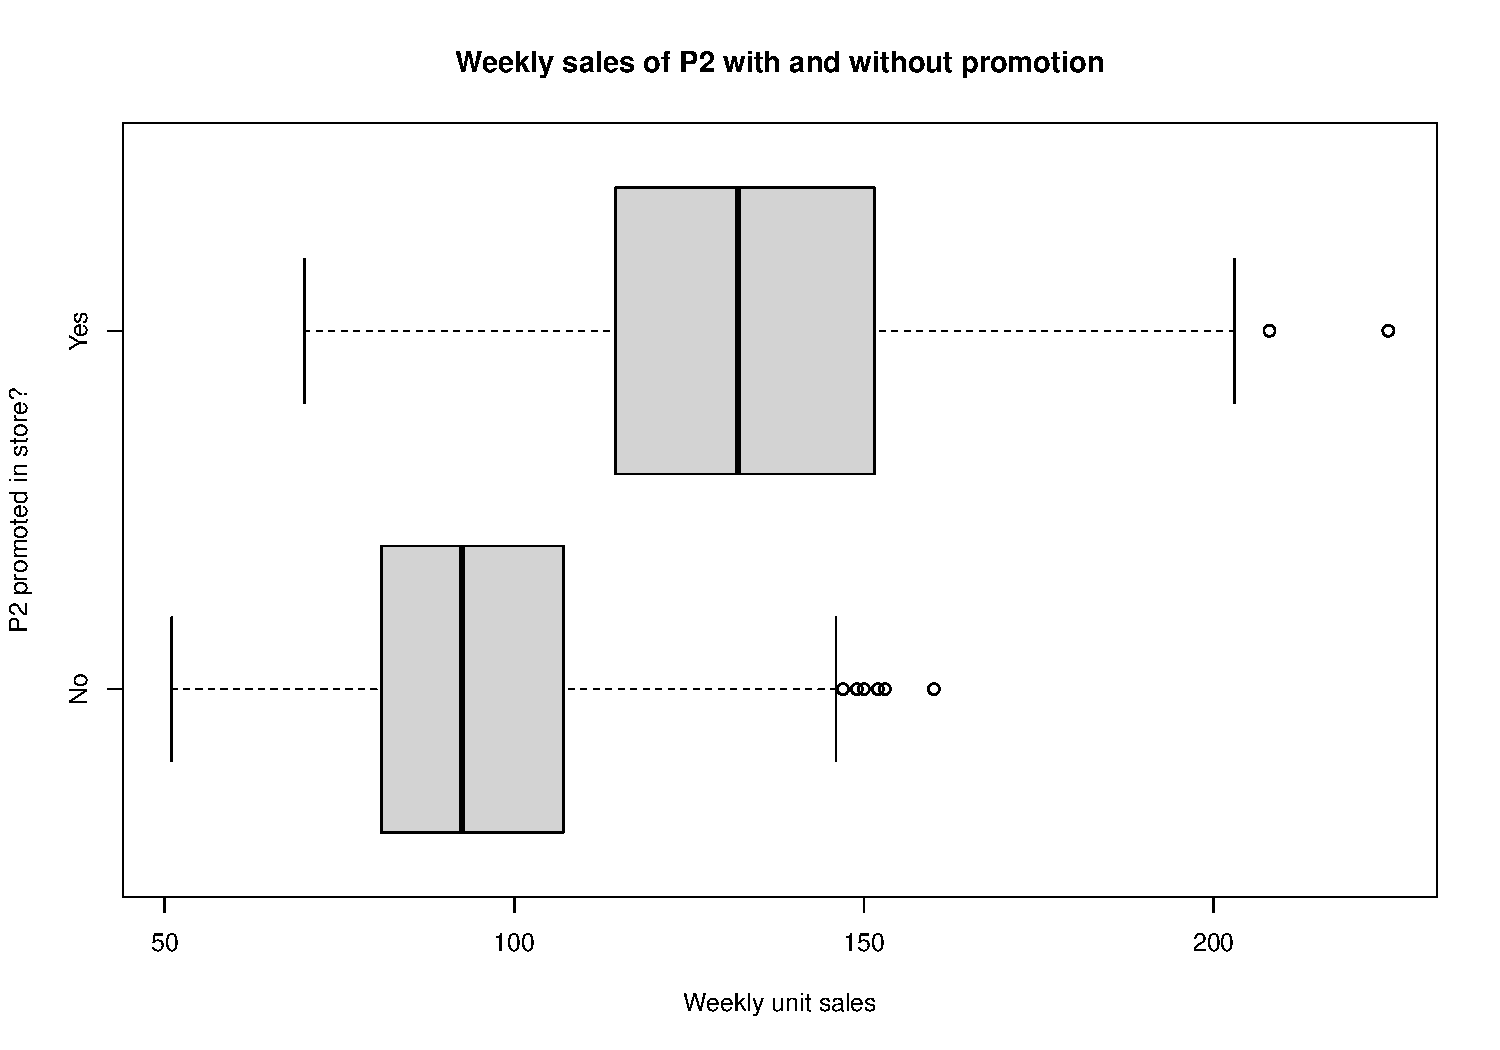
\includegraphics[width=0.5\textwidth,height=\textheight]{003_describing_data_files/figure-beamer/unnamed-chunk-22-1.pdf}
\end{center}
\end{frame}

\begin{frame}[fragile]{}
\phantomsection\label{section-24}
\begin{itemize}
\item
  \textbf{Boxplots: the tidyverse way}

  \begin{itemize}
  \tightlist
  \item
    Boxplot product 2 sales by promotion
  \end{itemize}
\end{itemize}

\tiny

\begin{Shaded}
\begin{Highlighting}[]
\NormalTok{weekly\_store }\SpecialCharTok{|\textgreater{}} \FunctionTok{ggplot}\NormalTok{()}
\end{Highlighting}
\end{Shaded}

\begin{center}

\includegraphics[width=0.5\textwidth,height=\textheight]{003_describing_data_files/figure-beamer/unnamed-chunk-23-1.pdf}
\end{center}
\end{frame}

\begin{frame}[fragile]{}
\phantomsection\label{section-25}
\begin{itemize}
\item
  \textbf{Boxplots: the tidyverse way}

  \begin{itemize}
  \tightlist
  \item
    Boxplot product 2 sales by promotion
  \end{itemize}
\end{itemize}

\tiny

\begin{Shaded}
\begin{Highlighting}[]
\NormalTok{weekly\_store }\SpecialCharTok{|\textgreater{}} \FunctionTok{ggplot}\NormalTok{() }\SpecialCharTok{+} 
  \FunctionTok{geom\_boxplot}\NormalTok{(}\FunctionTok{aes}\NormalTok{(}\AttributeTok{x =}\NormalTok{ p2sales, }\AttributeTok{y =}\NormalTok{ p2prom))}
\end{Highlighting}
\end{Shaded}

\begin{center}
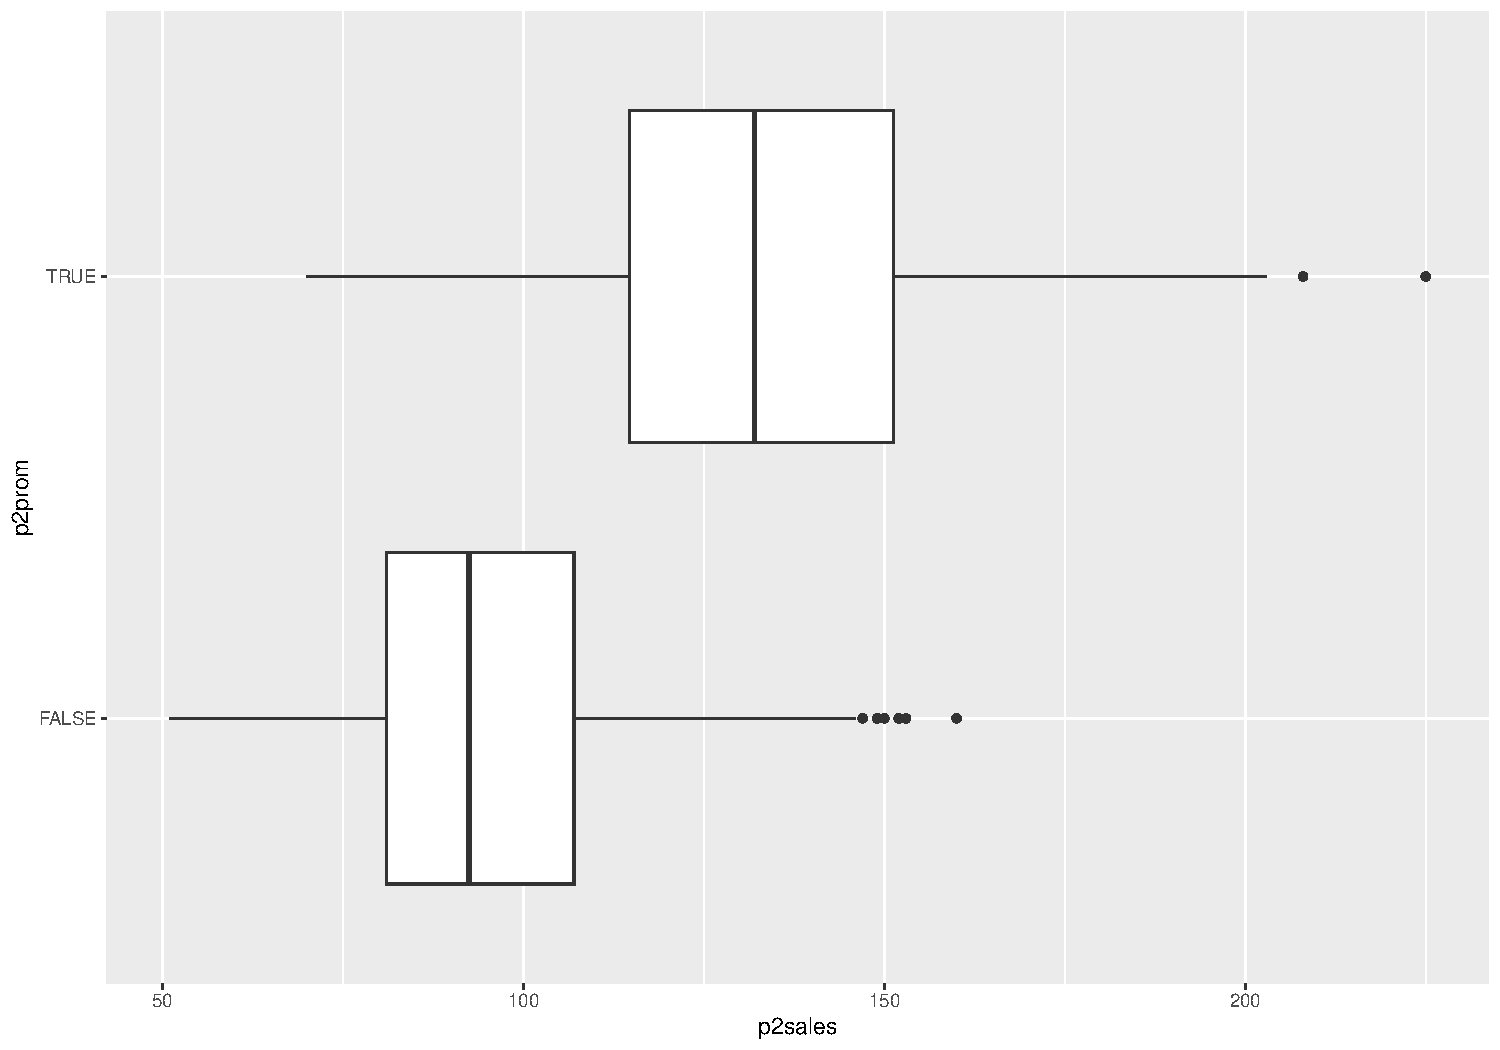
\includegraphics[width=0.5\textwidth,height=\textheight]{003_describing_data_files/figure-beamer/unnamed-chunk-24-1.pdf}
\end{center}
\end{frame}

\begin{frame}[fragile]{}
\phantomsection\label{section-26}
\begin{itemize}
\item
  \textbf{Boxplots: the tidyverse way}

  \begin{itemize}
  \tightlist
  \item
    Boxplot product 2 sales by promotion
  \end{itemize}
\end{itemize}

\tiny

\begin{Shaded}
\begin{Highlighting}[]
\NormalTok{weekly\_store }\SpecialCharTok{|\textgreater{}} \FunctionTok{ggplot}\NormalTok{() }\SpecialCharTok{+} 
  \FunctionTok{geom\_boxplot}\NormalTok{(}\FunctionTok{aes}\NormalTok{(}\AttributeTok{x =}\NormalTok{ p2sales, }\AttributeTok{y =}\NormalTok{ p2prom)) }\SpecialCharTok{+} 
  \FunctionTok{scale\_y\_discrete}\NormalTok{(}\AttributeTok{labels =} \FunctionTok{c}\NormalTok{(}\StringTok{"No"}\NormalTok{, }\StringTok{"Yes"}\NormalTok{))}
\end{Highlighting}
\end{Shaded}

\begin{center}
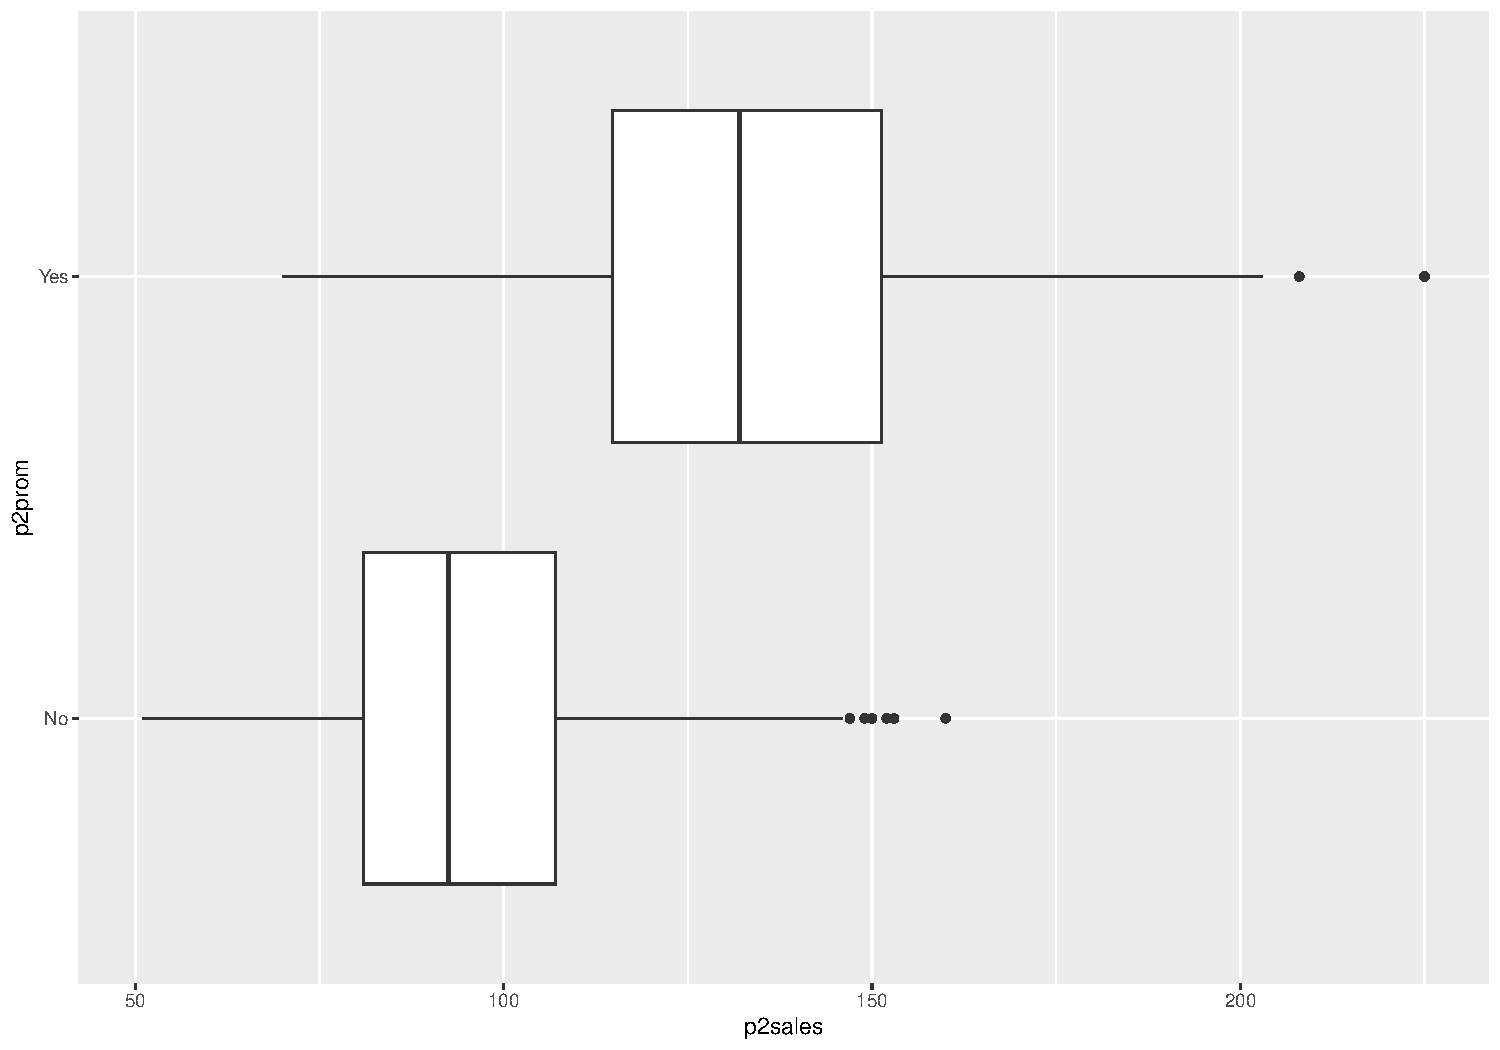
\includegraphics[width=0.5\textwidth,height=\textheight]{003_describing_data_files/figure-beamer/unnamed-chunk-25-1.pdf}
\end{center}
\end{frame}

\begin{frame}[fragile]{}
\phantomsection\label{section-27}
\begin{itemize}
\item
  \textbf{Boxplots: the tidyverse way}

  \begin{itemize}
  \tightlist
  \item
    Boxplot product 2 sales by promotion
  \end{itemize}
\end{itemize}

\tiny

\begin{Shaded}
\begin{Highlighting}[]
\NormalTok{weekly\_store }\SpecialCharTok{|\textgreater{}} \FunctionTok{ggplot}\NormalTok{() }\SpecialCharTok{+} 
  \FunctionTok{geom\_boxplot}\NormalTok{(}\FunctionTok{aes}\NormalTok{(}\AttributeTok{x =}\NormalTok{ p2sales, }\AttributeTok{y =}\NormalTok{ p2prom)) }\SpecialCharTok{+} 
  \FunctionTok{scale\_y\_discrete}\NormalTok{(}\AttributeTok{labels =} \FunctionTok{c}\NormalTok{(}\StringTok{"No"}\NormalTok{, }\StringTok{"Yes"}\NormalTok{)) }\SpecialCharTok{+}
  \FunctionTok{labs}\NormalTok{(}\AttributeTok{x =} \StringTok{"Weekly unit sales"}\NormalTok{, }\AttributeTok{y =} \StringTok{"P2 promoted in store?"}\NormalTok{, }
       \AttributeTok{title =} \StringTok{"Weekly sales of P2 with and without promotion"}\NormalTok{)}
\end{Highlighting}
\end{Shaded}

\begin{center}
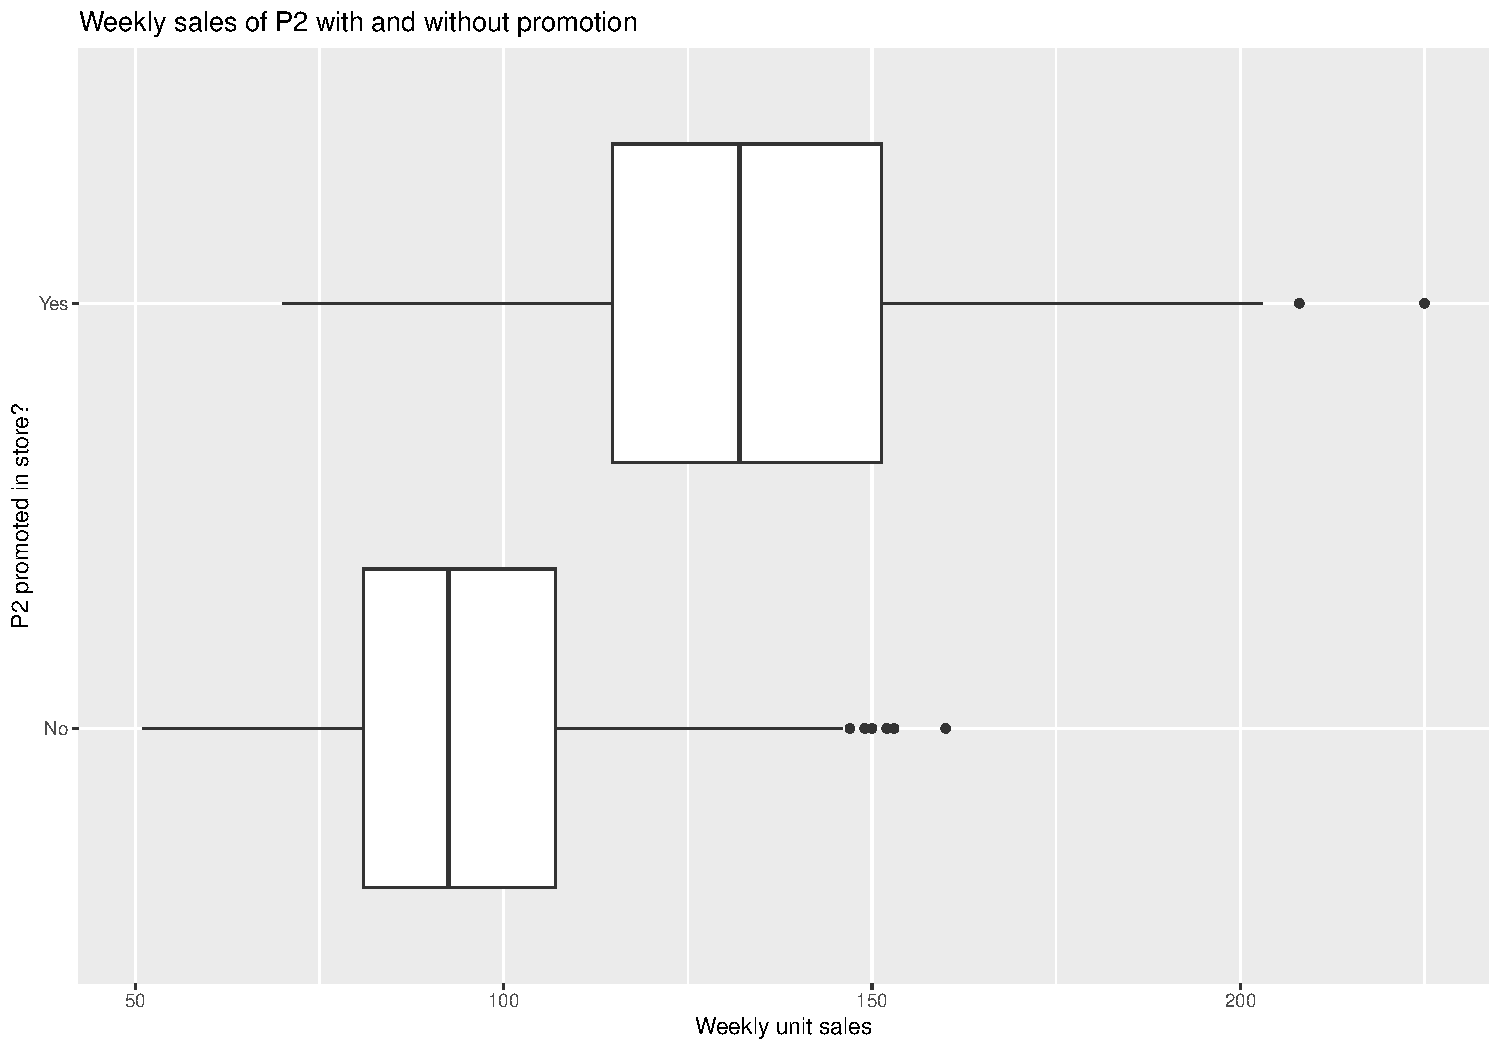
\includegraphics[width=0.5\textwidth,height=\textheight]{003_describing_data_files/figure-beamer/unnamed-chunk-26-1.pdf}
\end{center}
\end{frame}

\section{Questions and answers with
data}\label{questions-and-answers-with-data}

\begin{frame}[fragile]{}
\phantomsection\label{section-28}
\begin{itemize}
\item
  \textbf{In what countries the company sell more units of product 2?}

  \begin{itemize}
  \tightlist
  \item
    Preparing the data
  \end{itemize}
\end{itemize}

\tiny

\begin{Shaded}
\begin{Highlighting}[]
\NormalTok{weekly\_store\_sales\_by\_country }\OtherTok{\textless{}{-}}\NormalTok{ weekly\_store }\SpecialCharTok{|\textgreater{}} 
  \FunctionTok{group\_by}\NormalTok{(country)}
\NormalTok{weekly\_store\_sales\_by\_country}
\end{Highlighting}
\end{Shaded}

\begin{verbatim}
# A tibble: 2,080 x 10
# Groups:   country [7]
   storeNum Year  Week  p1sales p2sales p1price p2price p1prom p2prom country
   <fct>    <ord> <ord>   <dbl>   <dbl>   <dbl>   <dbl> <lgl>  <lgl>  <chr>  
 1 101      1     1         127     106    2.29    2.29 FALSE  FALSE  US     
 2 101      1     2         137     105    2.49    2.49 FALSE  FALSE  US     
 3 101      1     3         156      97    2.99    2.99 TRUE   FALSE  US     
 4 101      1     4         117     106    2.99    3.19 FALSE  FALSE  US     
 5 101      1     5         138     100    2.49    2.59 FALSE  TRUE   US     
 6 101      1     6         115     127    2.79    2.49 FALSE  FALSE  US     
 7 101      1     7         116      90    2.99    3.19 FALSE  FALSE  US     
 8 101      1     8         106     126    2.99    2.29 FALSE  FALSE  US     
 9 101      1     9         116      94    2.29    2.29 FALSE  FALSE  US     
10 101      1     10        145      91    2.49    2.99 FALSE  FALSE  US     
# i 2,070 more rows
\end{verbatim}
\end{frame}

\begin{frame}[fragile]{}
\phantomsection\label{section-29}
\begin{itemize}
\item
  \textbf{In what countries the company sell more units of product 2?}

  \begin{itemize}
  \tightlist
  \item
    Preparing the data
  \end{itemize}
\end{itemize}

\tiny

\begin{Shaded}
\begin{Highlighting}[]
\NormalTok{weekly\_store\_sales\_by\_country }\OtherTok{\textless{}{-}}\NormalTok{ weekly\_store }\SpecialCharTok{|\textgreater{}} 
  \FunctionTok{group\_by}\NormalTok{(country) }\SpecialCharTok{|\textgreater{}}
  \FunctionTok{summarise}\NormalTok{(}\AttributeTok{sum\_p2sales =} \FunctionTok{sum}\NormalTok{(p2sales))}
\NormalTok{weekly\_store\_sales\_by\_country}
\end{Highlighting}
\end{Shaded}

\begin{verbatim}
# A tibble: 7 x 2
  country sum_p2sales
  <chr>         <dbl>
1 AU             9934
2 BR            21362
3 CN            20911
4 DE            52263
5 GB            31264
6 JP            41344
7 US            31248
\end{verbatim}
\end{frame}

\begin{frame}[fragile]{}
\phantomsection\label{section-30}
\begin{itemize}
\item
  \textbf{In what countries the company sell more units of product 2?}

  \begin{itemize}
  \tightlist
  \item
    Preparing the data
  \end{itemize}
\end{itemize}

\tiny

\begin{Shaded}
\begin{Highlighting}[]
\NormalTok{weekly\_store\_sales\_by\_country }\OtherTok{\textless{}{-}}\NormalTok{ weekly\_store }\SpecialCharTok{|\textgreater{}} 
  \FunctionTok{group\_by}\NormalTok{(country) }\SpecialCharTok{|\textgreater{}}
  \FunctionTok{summarise}\NormalTok{(}\AttributeTok{sum\_p2sales =} \FunctionTok{sum}\NormalTok{(p2sales)) }\SpecialCharTok{|\textgreater{}}
  \FunctionTok{mutate}\NormalTok{(}\AttributeTok{country =} \FunctionTok{fct\_reorder}\NormalTok{(}\AttributeTok{.f =}\NormalTok{ country, }\AttributeTok{.x =}\NormalTok{ sum\_p2sales))}
\NormalTok{weekly\_store\_sales\_by\_country}
\end{Highlighting}
\end{Shaded}

\begin{verbatim}
# A tibble: 7 x 2
  country sum_p2sales
  <fct>         <dbl>
1 AU             9934
2 BR            21362
3 CN            20911
4 DE            52263
5 GB            31264
6 JP            41344
7 US            31248
\end{verbatim}
\end{frame}

\begin{frame}[fragile]{}
\phantomsection\label{section-31}
\begin{itemize}
\item
  \textbf{In what countries the company sell more units of product 2?}

  \begin{itemize}
  \tightlist
  \item
    Visualizing data
  \end{itemize}
\end{itemize}

\tiny

\begin{Shaded}
\begin{Highlighting}[]
\NormalTok{weekly\_store\_sales\_by\_country }\SpecialCharTok{|\textgreater{}} \FunctionTok{ggplot}\NormalTok{()}
\end{Highlighting}
\end{Shaded}

\begin{center}

\includegraphics[width=0.5\textwidth,height=\textheight]{003_describing_data_files/figure-beamer/unnamed-chunk-30-1.pdf}
\end{center}
\end{frame}

\begin{frame}[fragile]{}
\phantomsection\label{section-32}
\begin{itemize}
\item
  \textbf{In what countries the company sell more units of product 2?}

  \begin{itemize}
  \tightlist
  \item
    Visualizing data
  \end{itemize}
\end{itemize}

\tiny

\begin{Shaded}
\begin{Highlighting}[]
\NormalTok{weekly\_store\_sales\_by\_country }\SpecialCharTok{|\textgreater{}} \FunctionTok{ggplot}\NormalTok{() }\SpecialCharTok{+} 
  \FunctionTok{geom\_col}\NormalTok{(}\FunctionTok{aes}\NormalTok{(}\AttributeTok{x =}\NormalTok{ country, }\AttributeTok{y =}\NormalTok{ sum\_p2sales))}
\end{Highlighting}
\end{Shaded}

\begin{center}
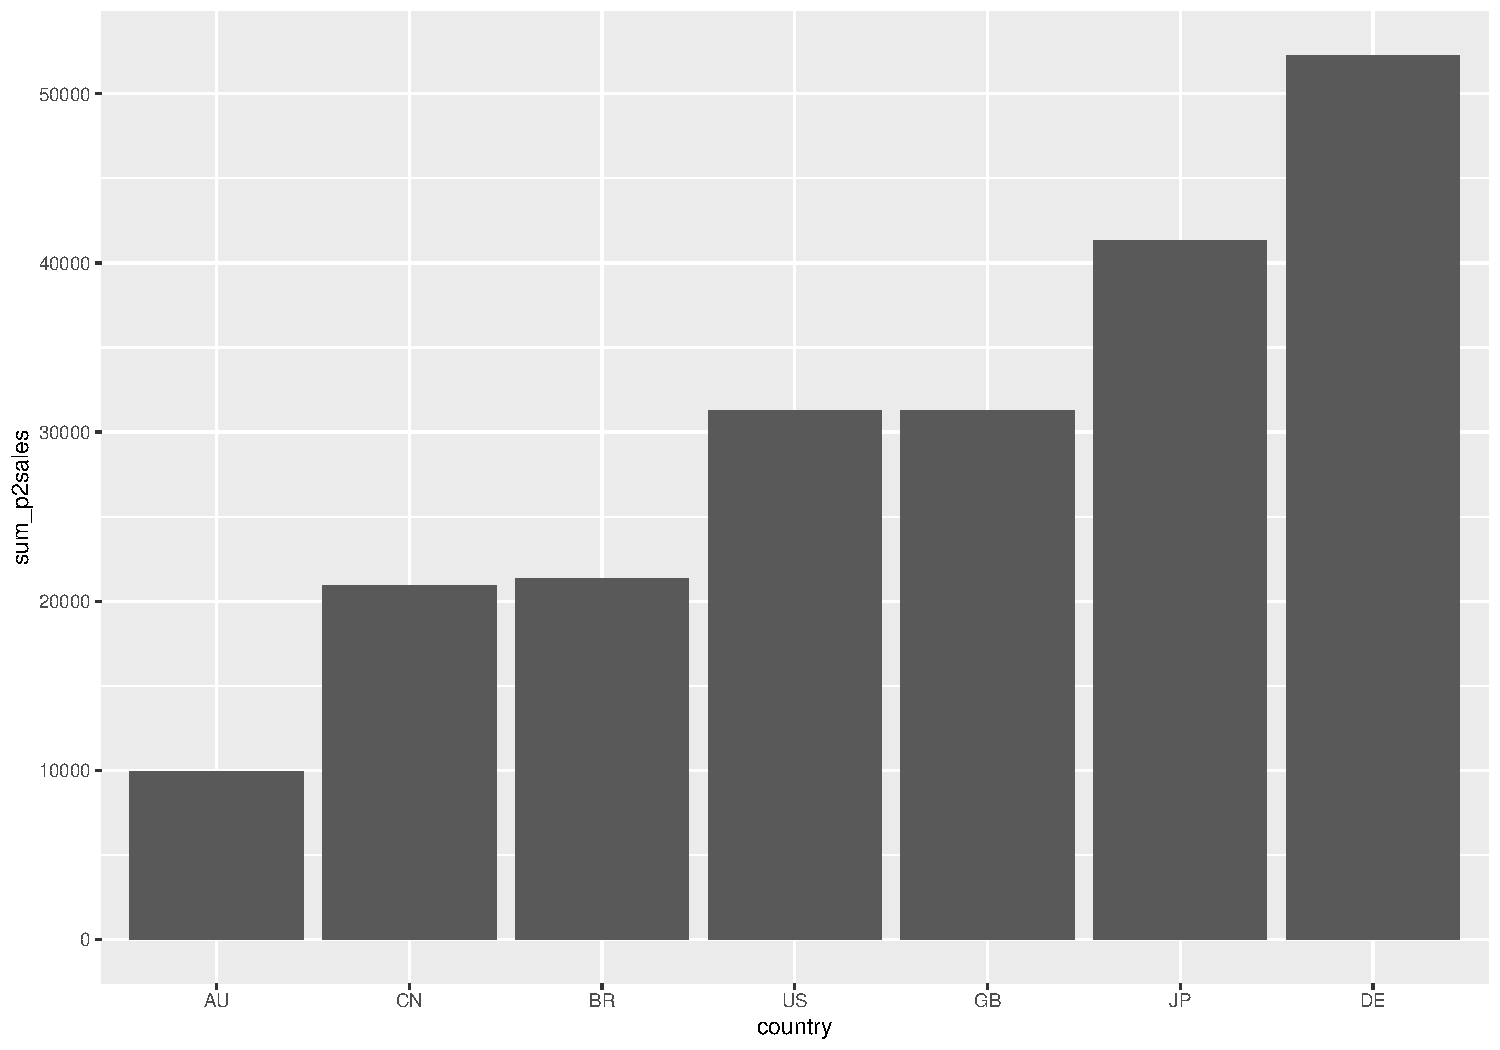
\includegraphics[width=0.5\textwidth,height=\textheight]{003_describing_data_files/figure-beamer/unnamed-chunk-31-1.pdf}
\end{center}
\end{frame}

\begin{frame}[fragile]{}
\phantomsection\label{section-33}
\begin{itemize}
\item
  \textbf{In what countries the company sell more units of product 2?}

  \begin{itemize}
  \tightlist
  \item
    Visualizing data
  \end{itemize}
\end{itemize}

\tiny

\begin{Shaded}
\begin{Highlighting}[]
\NormalTok{weekly\_store\_sales\_by\_country }\SpecialCharTok{|\textgreater{}} \FunctionTok{ggplot}\NormalTok{() }\SpecialCharTok{+} 
  \FunctionTok{geom\_col}\NormalTok{(}\FunctionTok{aes}\NormalTok{(}\AttributeTok{x =}\NormalTok{ country, }\AttributeTok{y =}\NormalTok{ sum\_p2sales, }\AttributeTok{fill =}\NormalTok{ country),}
           \AttributeTok{color =} \StringTok{"black"}\NormalTok{, }\AttributeTok{show.legend =} \ConstantTok{FALSE}\NormalTok{)}
\end{Highlighting}
\end{Shaded}

\begin{center}
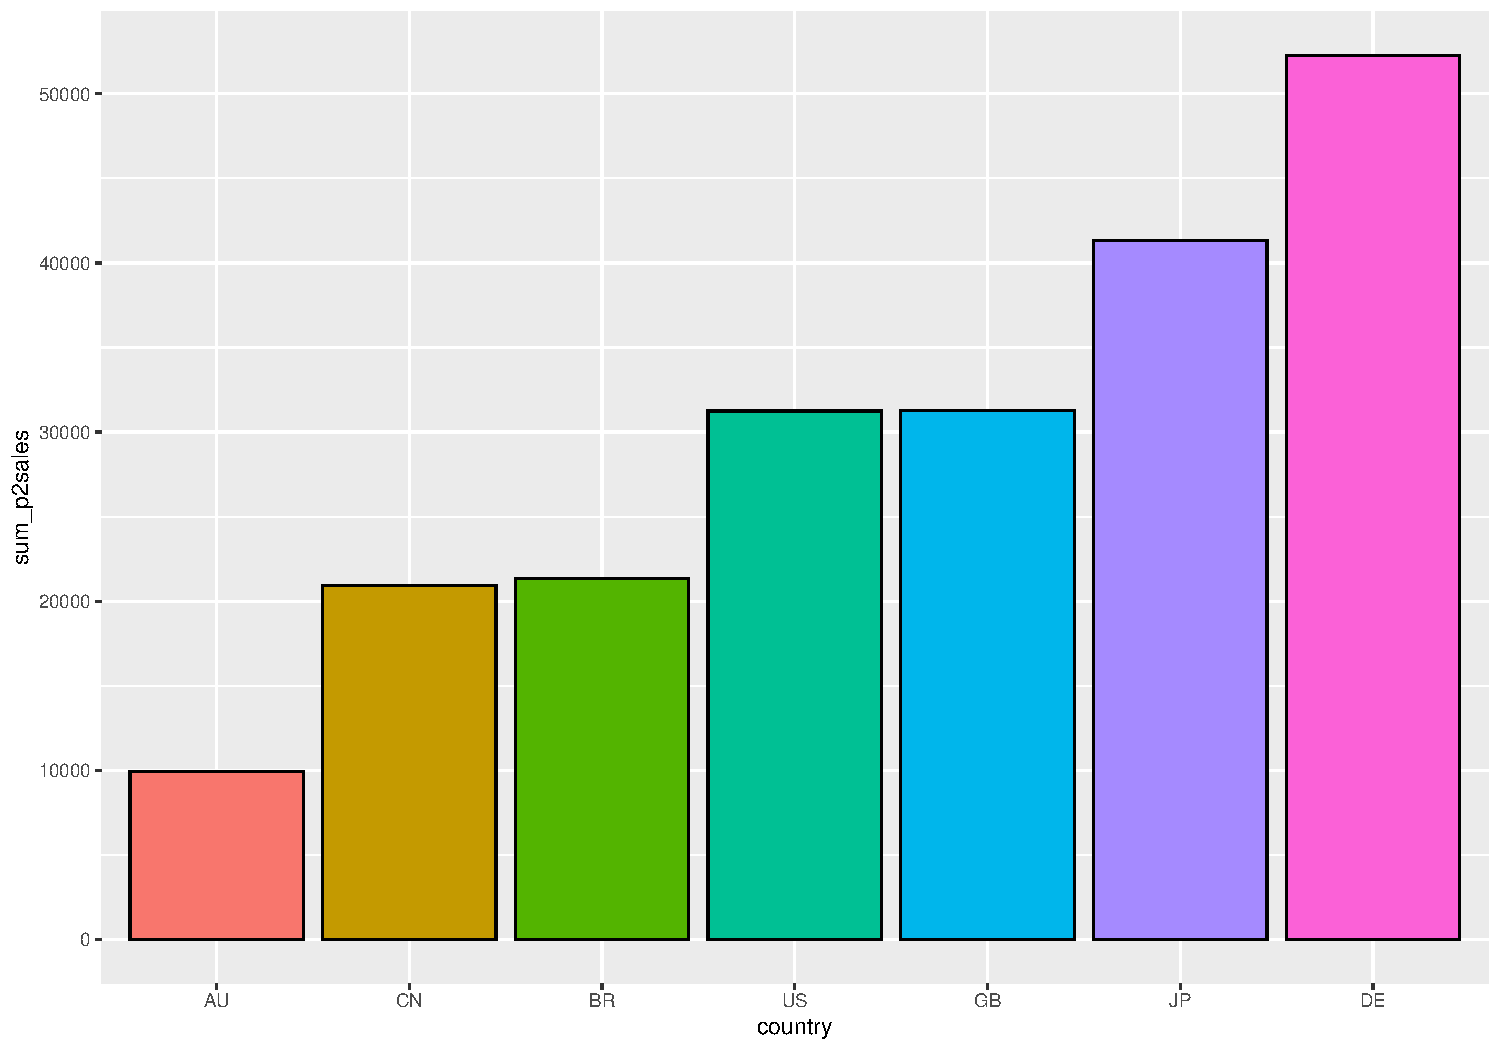
\includegraphics[width=0.5\textwidth,height=\textheight]{003_describing_data_files/figure-beamer/unnamed-chunk-32-1.pdf}
\end{center}
\end{frame}

\begin{frame}[fragile]{}
\phantomsection\label{section-34}
\begin{itemize}
\item
  \textbf{In what countries the company sell more units of product 2?}

  \begin{itemize}
  \tightlist
  \item
    Visualizing data
  \end{itemize}
\end{itemize}

\tiny

\begin{Shaded}
\begin{Highlighting}[]
\NormalTok{weekly\_store\_sales\_by\_country }\SpecialCharTok{|\textgreater{}} \FunctionTok{ggplot}\NormalTok{() }\SpecialCharTok{+} 
  \FunctionTok{geom\_col}\NormalTok{(}\FunctionTok{aes}\NormalTok{(}\AttributeTok{x =}\NormalTok{ country, }\AttributeTok{y =}\NormalTok{ sum\_p2sales, }\AttributeTok{fill =}\NormalTok{ country),}
           \AttributeTok{color =} \StringTok{"black"}\NormalTok{, }\AttributeTok{show.legend =} \ConstantTok{FALSE}\NormalTok{) }\SpecialCharTok{+}
  \FunctionTok{scale\_x\_discrete}\NormalTok{(}\AttributeTok{labels =} \FunctionTok{c}\NormalTok{(}\StringTok{"Australia"}\NormalTok{, }\StringTok{"Japan"}\NormalTok{, }\StringTok{"Brazil"}\NormalTok{, }
                              \StringTok{"Britain"}\NormalTok{, }\StringTok{"Germany"}\NormalTok{, }\StringTok{"China"}\NormalTok{, }\StringTok{"United States"}\NormalTok{))}
\end{Highlighting}
\end{Shaded}

\begin{center}
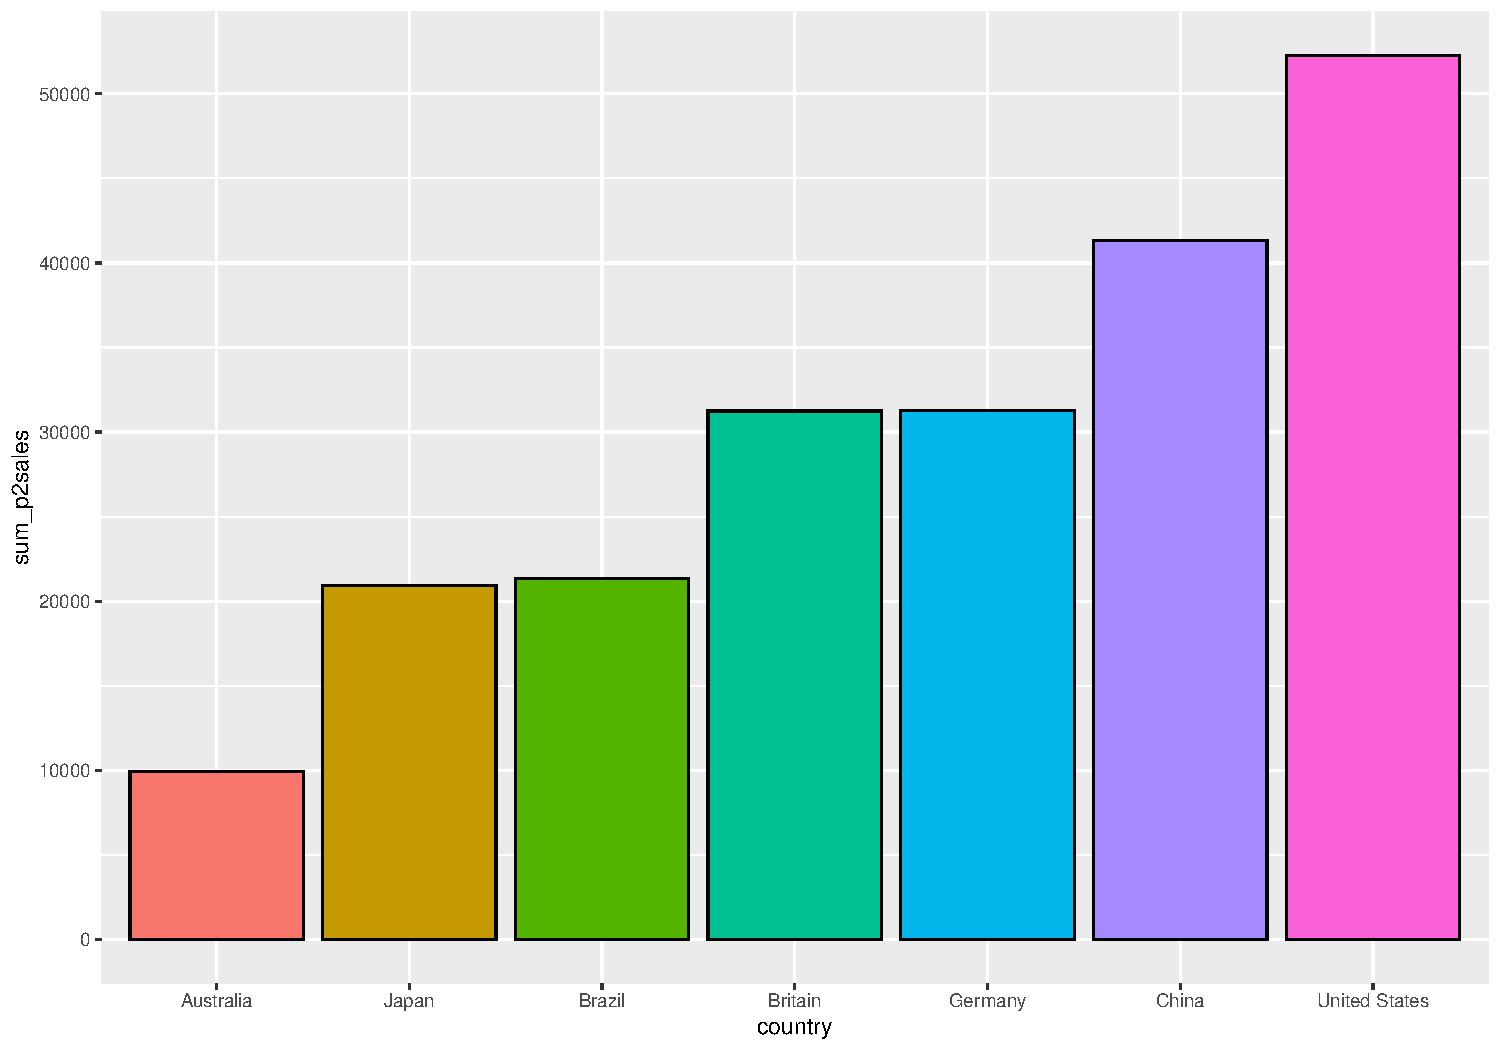
\includegraphics[width=0.5\textwidth,height=\textheight]{003_describing_data_files/figure-beamer/unnamed-chunk-33-1.pdf}
\end{center}
\end{frame}

\begin{frame}[fragile]{}
\phantomsection\label{section-35}
\begin{itemize}
\item
  \textbf{In what countries the company sell more units of product 2?}

  \begin{itemize}
  \tightlist
  \item
    Visualizing data
  \end{itemize}
\end{itemize}

\tiny

\begin{Shaded}
\begin{Highlighting}[]
\NormalTok{weekly\_store\_sales\_by\_country }\SpecialCharTok{|\textgreater{}} \FunctionTok{ggplot}\NormalTok{() }\SpecialCharTok{+} 
  \FunctionTok{geom\_col}\NormalTok{(}\FunctionTok{aes}\NormalTok{(}\AttributeTok{x =}\NormalTok{ country, }\AttributeTok{y =}\NormalTok{ sum\_p2sales, }\AttributeTok{fill =}\NormalTok{ country),}
           \AttributeTok{color =} \StringTok{"black"}\NormalTok{, }\AttributeTok{show.legend =} \ConstantTok{FALSE}\NormalTok{) }\SpecialCharTok{+}
  \FunctionTok{scale\_x\_discrete}\NormalTok{(}\AttributeTok{labels =} \FunctionTok{c}\NormalTok{(}\StringTok{"Australia"}\NormalTok{, }\StringTok{"Japan"}\NormalTok{, }\StringTok{"Brazil"}\NormalTok{, }
                              \StringTok{"Britain"}\NormalTok{, }\StringTok{"Germany"}\NormalTok{, }\StringTok{"China"}\NormalTok{, }\StringTok{"United States"}\NormalTok{)) }\SpecialCharTok{+}
  \FunctionTok{labs}\NormalTok{(}\AttributeTok{x =} \ConstantTok{NULL}\NormalTok{, }\AttributeTok{y =} \StringTok{"Sales (Units)"}\NormalTok{,}
       \AttributeTok{title =} \StringTok{"Sales in units per country"}\NormalTok{)}
\end{Highlighting}
\end{Shaded}

\begin{center}
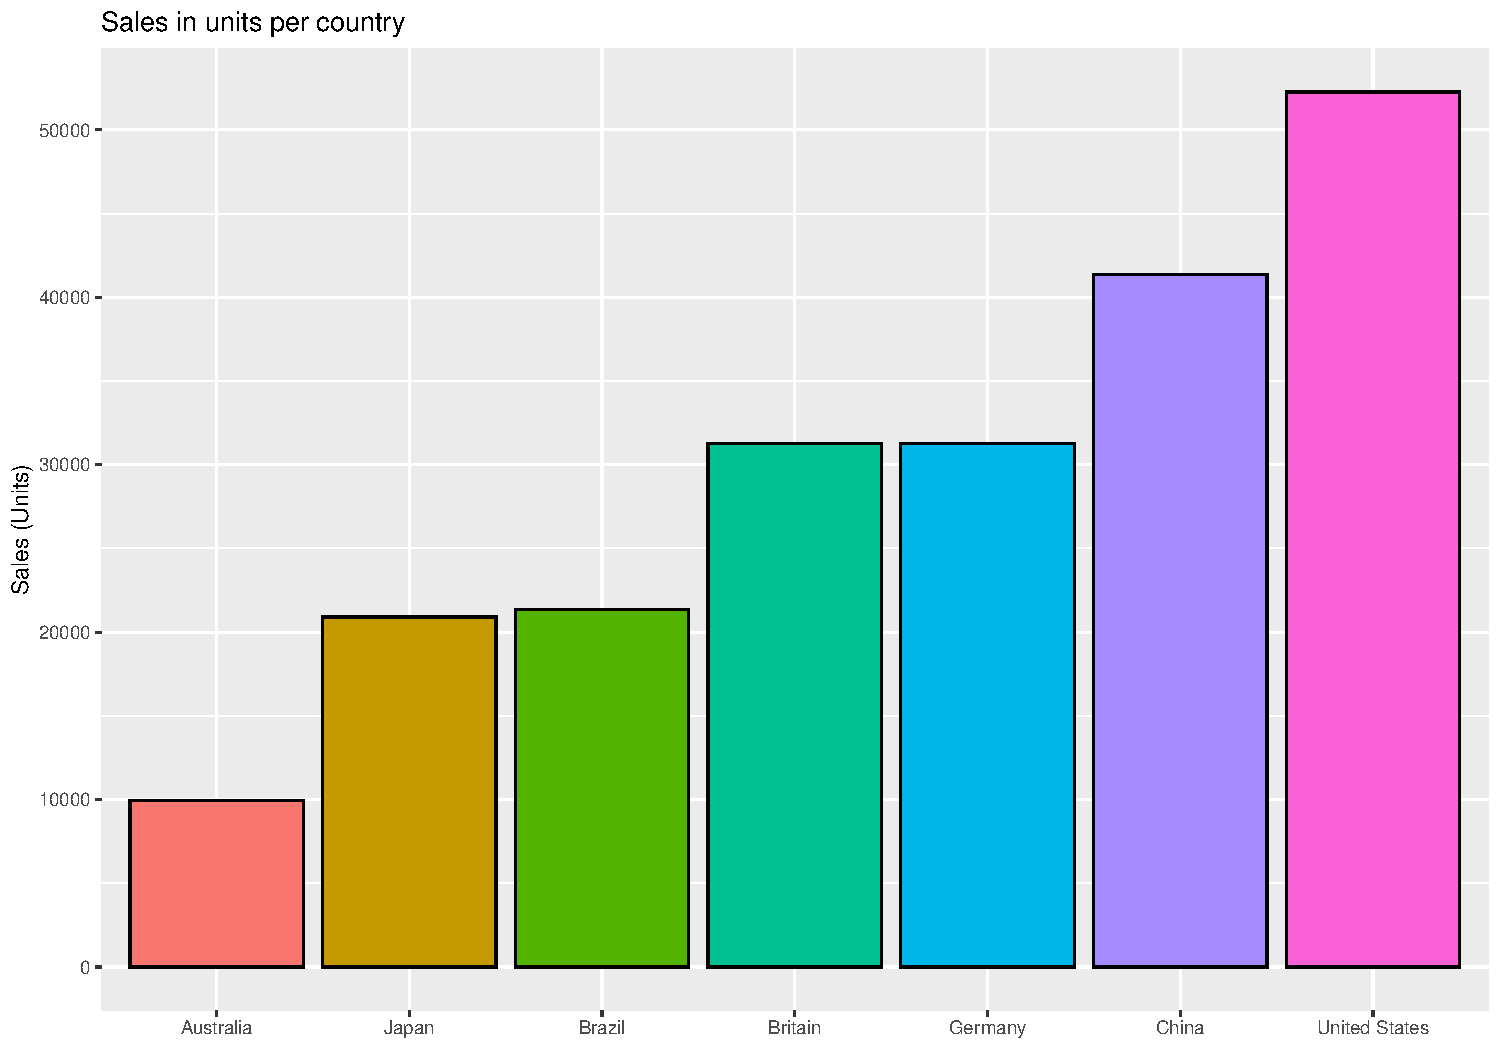
\includegraphics[width=0.5\textwidth,height=\textheight]{003_describing_data_files/figure-beamer/unnamed-chunk-34-1.pdf}
\end{center}
\end{frame}

\section{Acknowledgments}\label{acknowledgments}

\begin{frame}{}
\phantomsection\label{section-36}
\begin{itemize}
\item
  To my family that supports me
\item
  To the taxpayers of Colombia and the
  \href{https://www.umng.edu.co/estudiante}{\textbf{UMNG students}} who
  pay my salary
\item
  To the \href{https://www.business-science.io/}{\textbf{Business
  Science}} and \href{https://www.rfordatasci.com/}{\textbf{R4DS Online
  Learning}} communities where I learn
  \href{https://www.r-project.org/about.html}{\textbf{R}} and
  \href{https://www.python.org/about/}{\textbf{\(\pi\)-thon}}
\item
  To the \href{https://www.r-project.org/contributors.html}{\textbf{R
  Core Team}}, the creators of
  \href{https://posit.co/products/open-source/rstudio/}{\textbf{RStudio
  IDE}}, \href{https://quarto.org/}{\textbf{Quarto}} and the authors and
  maintainers of the packages
  \href{https://CRAN.R-project.org/package=tidyverse}{\textbf{tidyverse}},
  \href{https://CRAN.R-project.org/package=skimr}{\textbf{skimr}} and
  \href{https://CRAN.R-project.org/package=tinytex}{\textbf{tinytex}}
  for allowing me to access these tools without paying for a license
\item
  To the \href{https://www.kernel.org/category/about.html}{\textbf{Linux
  kernel community}} for allowing me the possibility to use some
  \href{https://static.lwn.net/Distributions/}{\textbf{Linux
  distributions}} as my main
  \href{https://en.wikipedia.org/wiki/Operating_system}{\textbf{OS}}
  without paying for a license
\end{itemize}
\end{frame}

\section*{References}\label{references}
\addcontentsline{toc}{section}{References}

\begin{frame}[allowframebreaks]{References}
\phantomsection\label{refs}
\begin{CSLReferences}{1}{0}
\bibitem[\citeproctext]{ref-chapman_r_2019}
Chapman, Chris, and Elea McDonnell Feit. 2019. \emph{R {For} {Marketing}
{Research} and {Analytics}}. 2nd ed. 2019. Use {R}! Cham: Springer
International Publishing : Imprint: Springer.
\url{https://doi-org.ezproxy.umng.edu.co/10.1007/978-3-030-14316-9}.

\end{CSLReferences}
\end{frame}




\end{document}
